% ------------------------------------------------------------------------
% ------------------------------------------------------------------------
% ICMC: Modelo de Trabalho Acadêmico (tese de doutorado, dissertação de
% mestrado e trabalhos monográficos em geral) em conformidade com 
% ABNT NBR 14724:2011: Informação e documentação - Trabalhos acadêmicos -
% Apresentação
% ------------------------------------------------------------------------
% ------------------------------------------------------------------------

% Opções: 
%   Qualificação         = qualificacao 
%   Curso                = doutorado/mestrado
%   Situação do trabalho = pre-defesa/pos-defesa (exceto para qualificação)
% -- opções do pacote babel --
% Idioma padrão = brazil
	%spanish,			% idioma adicional para hifenização
	%english,			% idioma adicional para hifenização
	%brazil				% o último idioma é o principal do documento
\documentclass[mestrado, pre-defesa, spanish, english, brazil]{../packages/icmc}
	
% ---
% Pacotes Opcionais
% ---
\usepackage{rotating}           % Usado para rotacionar o texto
\usepackage[all,knot,arc,import,poly]{xy}   % Pacote para desenhos gráficos
% Este pacote pode conflitar com outros pacotes gráficos como o ``pictex''
% Então é necessário usar apenas um dos pacotes conflitantes
%\usepackage[usenames,dvipsnames]{color}
\usepackage{graphicx,pifont}
\usepackage{listings}
\usepackage{subcaption}

\let\oldding\ding% Store old \ding in \oldding
\renewcommand{\ding}[2][1]{\scalebox{#1}{\oldding{#2}}}% Scale \oldding via optional argument

\newcommand{\VerbL}{0.52\textwidth}
\newcommand{\LatL}{0.42\textwidth}

%\newcommand{\thereIs}{\textcolor{OliveGreen}{\ding[1.5]{52}}}
%\newcommand{\thereNotIs}{\textcolor{red}{\ding[1.5]{55}}}
\newcommand{\thereIs}{\ding[1.5]{52}}
\newcommand{\thereNotIs}{\ding[1.5]{55}}


% ---
% Informações de dados para CAPA e FOLHA DE ROSTO
% ---
\titulo{Extensão da geração de carga do Bench4Q para Benchmark de Desempenho em Regime Transiente.}
\autor[Souza, F. L.]{Flavio Luiz dos Santos de Souza}
\orientador[Orientador]{Prof. Dr.}{Francisco José Monaco}
%\coorientador{Prof. Dr.}{Fulano de Tal}
\curso{CCMC}
\data{\the\day}{\the\month}{\the\year} % Data do depósito
% ---
  

% ---
% RESUMOS
% ---

% Resumo em português
% conter no máximo 500 palavras
\textoresumo{
    Este trabalho de mestrado apresenta o desenvolvimento de uma extensão no \textit{benchmark} Bench4Q. Este \textit{benchmark} é utilizado para gerar carga sintética a um sistema \textit{e-commerce} acoplado no \textit{benchmark}. Seu principal emprego na literatura têm sido em avaliação de desempenho sob carga estacionária.  Contudo, recentes pesquisas  tem apresentado interesse no estudo de arquiteturas adaptativas de autogerenciamento de recursos, o que implica em responder à perturbações e atender a requisitos de desempenho em regime transiente.  No entanto, este \textit{benchmark} não trata os estados transiente do sistema. Este trabalho tem por objetivo estender o \textit{benchmark} Bench4Q acrescentando-lhe capacidades de excitar a resposta transiente do sistema mediante a perturbações da carga de trabalho.  Para isso, o software foi acrescido de funcionalidade capaz de gerenciar a modulação da carga de trabalho modulada. Os experimentos foram executados em um ambiente multicamadas que apresentou resultados satisfatórios ao objetivo, e apresentou contribuições para a área como a presença de dinâmica entre as camadas.
    }{Bench4Q, \textit{Benchmark}, Modelagem de Carga de trabalho, Sistemas Dinâmicos, Computação em Nuvem}

% ---
% resumo em inglês
% ---
\textoresumo[english]{
    The software package Bench4q is a benchmark for cloud computing applications which simulates various aspects of conventional architectures and workloads in this kind of environment. It is mainly referenced in the literature in works on performance evaluation under stationary load.  Recent research works have broaden its interest to the study of adaptive architectures of resource self-management, what implies in respond to disturbances and meet performance requirements in transient regime.  This work aims at extending Bench4q adding it capabilities to excite the transient response of the system by means of applying disturbances during execution time.  As for that, the piece of software shall be enriched with functionalities for generating non-stationary workload and programmed disturbances. The motivation of this piece of work, insertion in other ongoing research and directions are introduced. 
    }{Bench4Q, \textit{Benchmark}, \textit{Workload model}, \textit{Dynamic Systems}, \textit{Cloud Computing}}

% ---
% resumo em espanhol
% ---
%\textoresumo[spanish]{
%    Este trabajo es un breve modelo para la redacción de monografías de cualificación, disertaciones y tesis utilizando el ambiente LaTeX, de acuerdo a las normas exigidas por el Instituto de Ciencias Matemáticas y Computación (ICMC) de la Universidad de São Paulo (USP). Para la confección de este modelo fue utilizada la última versión (1.9.1) del paquete de clases abnTeX2 que sigue las normas de la Asociación Brasilera de Normas Técnicas. La elaboración de una monografía, disertación o tesis puede ser realizada reescribiendo el contenido de este modelo.
%    }{Template, Monografías de cualificación, Disertacion, Tesis, Latex}
    
    
% ---
% Configurações de aparência do PDF final
% ---
% alterando o aspecto da cor azul
\definecolor{blue}{RGB}{41,5,195}

% informações do PDF
\makeatletter
\hypersetup{
     	pagebackref=true,
		pdftitle={\@title}, 
		pdfauthor={\@author},
    	pdfsubject={\imprimirpreambulo},
	    pdfcreator={LaTeX with abnTeX2/ICMC-USP},
		pdfkeywords={\palavraschave}, 
		colorlinks=true,       		% false: boxed links; true: colored links
    	linkcolor=blue,          	% color of internal links
    	citecolor=blue,        		% color of links to bibliography
    	filecolor=magenta,      	% color of file links
		urlcolor=blue,
		bookmarksdepth=4
}
\makeatother
% --- 

% ----------------------------------------------------------
% ELEMENTOS PRÉ-TEXTUAIS
% ----------------------------------------------------------

% Inserir a ficha catalográfica
%\incluifichacatalografica*{tex/fichaCatalografica.pdf}
\incluifichacatalografica{634} % Código Cutter: número atribuído ao sobrenome do autor. Para obtê-lo, consulte a tabela Cutter Sanborn (em http://www.davignon.qc.ca/cutter1.html), procure pelo sobrenome ou forma mais próxima ao sobrenome completo e coloque o número indicado como parâmetro.


% DEDICATÓRIA / AGRADECIMENTO / EPÍGRAFE
%\textodedicatoria*{pre-textual/dedicatoria}
%\textoagradecimentos*{pre-textual/agradecimentos}
%\textoepigrafe*{pre-textual/epigrafe}

% Inclui a lista de figuras
\incluilistadefiguras

% Inclui a lista de tabelas
\incluilistadetabelas

% Inclui a lista de quadros
%\incluilistadequadros

% Inclui a lista de algoritmos
%\incluilistadealgoritmos

% Inclui a lista de códigos
\incluilistadecodigos

% Inclui a lista de siglas e abreviaturas
\incluilistadesiglas

% Inclui a lista de símbolos
%\incluilistadesimbolos

% ----
% Início do documento
% ----
\begin{document}
% ----------------------------------------------------------
% ELEMENTOS TEXTUAIS
% ----------------------------------------------------------
\textual

\chapter{Introdução}
\label{chapter:introducao}
\setcounter{page}{1}
Para além da pesquisa acadêmica, a Computação em Nuvem, hoje se faz presente na vida de pessoas e empresas, integrando-se em suas rotinas e atividades do cotidiano e estabelecendo-se como um importante e fundamental meio computacional. 

O conceito, Computação em Nuvem, tem se tornando um paradigma cada vez mais reconhecido e utilizado. Inúmeras empresas tem apoiado e incentivado o uso e o seu desenvolvimento, assim como o meio científico. Atualmente, os exemplos desse paradigma de computação oferecem diversas opções para armazenamento ou processamento de dados, tais como, a \textit{\sigla{S3}{Simple Storage Service}} da Amazon, Bigtable do Google, ou PNUTS do Yahoo \cite{Binnig2009}. \citeonline{vazquez2014} exemplificam o crescimento do Instagram, que construiu a sua base de usuários com mais de 150 milhões de usuários em menos de quatro anos usando soluções em nuvem.

O aumento da popularidade da Computação em Nuvem é impulsionado pelas vantagens oferecidas e pelo modelo dinamicamente escalável e o rápido desenvolvimento nos últimos anos levou a uma grande quantidade de publicações. O interesse no meio acadêmico e da indústria tem levado a uma quantidade considerável de publicações de artigos científicos nos últimos anos \cite{Heilig2014}. Como apresentado nos trabalhos de \citeonline{Heilig2014} e \citeonline{Yang2012}, o número de pesquisas tem concentrado esforços na resolução de problemas que em geral envolvem desempenho e/ou garantia de requisitos de Qualidade de Serviço (\textit{\sigla{QoS}{Quality of service}}). 

Nessa área existe uma grande preocupação por parte dos provedores de computação em garantir QoS de uma forma eficiente. Em termos de recursos, significa que os recursos virtuais (\textit{\sigla{VMs}{Virtual Machines}}) e/ou físicos devem ser alocados de forma autônoma, para que possam responder às influências externas, como a carga de trabalho. Observa-se, por outro lado, os \textit{data center} são muitas vezes subutilizados devido ao excesso de provisionamento de recursos, bem como as demandas de recursos que variam no tempo de acordo com os sistemas \cite{Padala2007}. \citeonline{Inomata2011} afirmam que tempo e dinheiro são investidos para projetar, construir, configurar, monitorar e manter recursos computacionais e que o futuro da Computação em Nuvem é o auto gerenciamento e a atribuição de recursos automáticos aos seus consumidores com base na carga de trabalho.

Atualmente, com o advento e crescimento das aplicações intensivas de dados, que lidam com grandes volumes em tempo real, a dinâmica do sistema passa ser apreciável, fenômeno frequentemente não perceptível claramente para os sistemas computacionais. Na prática, tais aplicações, de grande volume de dados, tendem a operarem com cargas de trabalho variante no tempo, causando inúmeras dificuldades. A Computação em Nuvem oferece uma infraestrutura elástica e escalável que pode ser utilizada para obter recursos sob demanda; no entanto, um problema em aberto é decidir sobre a correta alocação de recursos ao implantar um sistema na nuvem \cite{Cervino2012}. De modo geral, um sistema dinâmico não apresenta os efeitos das ações da carga de forma imediata. Por exemplo, a velocidade de um carro não atingem a sua velocidade máxima imediatamente ao acionamento do acelerador ou como a temperatura em uma sala muda instantaneamente quando um aquecedor é ligado.

Este comportamento, dinâmico, começa a ser apreciado em grandes sistemas computacionais, quando um súbito aumento de requisições para um \textit{website} em que os servidores não conseguem-se ajustar à demanda de modo imediato. 

O \textit{burstiness} (rajada) no fluxo de requisições é frequentemente encontrado em sistemas cliente-servidor. Esse \textit{burstiness} pode impactar de forma inesperada o desempenho de diferentes mecanismos de alocação de recursos projetados para o gerenciamento de um sistema adaptativo, e, portanto, testar e avaliar esses mecanismos sob cargas de trabalho reproduzíveis e controláveis é importante para o projeto do sistema.  Como ilustração, durante o evento promocional de um \textit{e-commerce} durante o \textit{Black Friday}, na edição de 2012, foi constatado que o tempo de resposta médio aos dias que antecederam 23 de Novembro de 2012, era de 5.3 segundos. A partir das 7 horas do dia evento, observou-se um aumento significativo no tempo de resposta conforme apresentado no gráfico da Figura \ref{fig:grafico-black-friday}. Mesmo hospedado em um ambiente de Computação em Nuvem, o sistema não teve a expectativa de que o volume de requisições aumentaria drasticamente, de tal maneira a prejudicar e comprometer os níveis de QoS, como tempo de respostas.

\begin{figure}[htb]
	\centering
	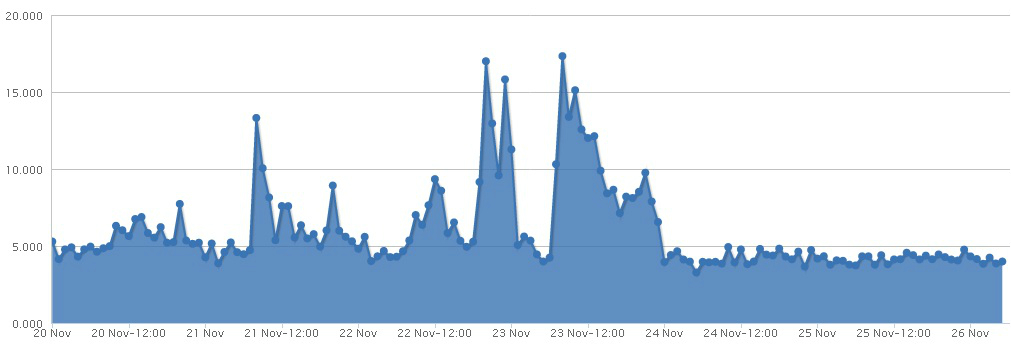
\includegraphics[scale=0.45]{grafico-black-friday.jpg}
	\caption{Tempo de resposta do \textit{Black Friday} Brasil 2012}
	\label{fig:grafico-black-friday}
	\fadaptada{blackfridayNews}
\end{figure}

As técnicas de gerenciamento de recursos são inúmeras, como as de inteligência artificial que utilizam lógica \textit{fuzzy}, algoritmos de mineração de dados e aprendizado de máquina \cite{Nobile2013}. As técnicas de aprendizado de máquina mostram-se interessantes para soluções imediatas, onde não há tempo hábil, inclusive, com abordagens não lineares empregadas para implementar um gerenciador de recursos responsável pela alteração dinâmica das capacidades computacionais. Outros trabalhos, como o \citeonline{Zhang2007}, buscam identificar padrões de comportamento na carga de trabalho e otimizar a provisão dinâmica dos recursos nas máquinas virtuais com base em algoritmos reativos. \citeonline{Quiroz2009} buscam detectar, por monitoramento, a padronização e a tendência da carga de trabalho com o objetivo de otimizar os recursos. \citeonline{Nobile2013} também propõe o uso de modelos de séries temporais para modelagem de tráfego de tempo real e previsão de demanda, que é usada para criar partições de conexões para diferentes classes de prioridade. \citeonline{Zhang2011}, utiliza de técnicas de estatística e avaliação dos recursos disponíveis para tomar a decisão de qual recurso deve ser alocado.

\citeonline{Dong2014} afirmam que atualmente a maioria das aplicações Web são concebidas com sistemas \textit{mult-tiers} (multi-camadas) devido à flexibilidade de escalabilidade.% O planejamento de capacidade é um passo importante para determinar a quantidade de recursos exigido para garantir determinada QoS. No entanto, em geral o planejamento de capacidade é basicamente uma decisão de longo prazo e quase estático, e os recursos são determinados pela taxa de utilização máxima da aplicação para evitar a pena excessiva de QoS.

\citeonline{Lourenco2015} afirmam que a partir de um planejamento de capacidade, e a gestão de recursos em tempo real aumenta a sofisticação da arquitetura da solução nos diversos níveis e complexidade, as abordagens convencionais para análise de sistemas computacionais modernos; e concluí que as dinâmicas emergentes das interligações desses sistemas \textit{mult-tiers} pode produzir efeitos transitórios sobre o desempenho, como resposta temporal, ou o amortecimento e/ou comportamento oscilatório. Uma vez que estes efeitos variáveis no tempo podem potencialmente afetar a capacidade de resposta, eficiência e até mesmo a estabilidade global, métodos e ferramentas para avaliação das propriedades dinâmicas de sistemas computacionais são de importância prática para fins da engenharia.

Há caso em que existe o interesse em controlar a dinâmica deste sistema, para tanto é necessário modelar o sistema em questão e projetar um controlador que manipulará a sua dinâmica. Para trabalhar com estes sistemas deve-se ser capaz de modelar a dinâmico do sistema, que em termos matemáticos é extrair um modelo matemático e analisar suas características dinâmicas. Um modelo matemático de um sistema dinâmico é definido como um conjunto de equações que representa a dinâmica de maneira relativamente razoável. Percebe-se que um modelo matemático não é exclusivo para um determinado sistema. Um sistema pode ser representando de muitas maneiras diferentes e, por conseguinte, podem ter diversos modelos matemáticos, dependendo da perspectiva, uns mais precisos que outros, e outros mais simplificados \cite{Ogata2001}.

Algumas vezes, é possível representar sistemas dinâmicos através de equações diferenciais obtidas com base nas leis básicas da física. Esses sistemas de equações diferenciais descrevem uma determinada dinâmica do sistema no domínio do tempo e, com o desenvolvimento dessas equações, é possível identificar propriedades fundamentais do sistema \cite{Nobile2013}. Quando a modelagem é muito dedutiva e muito complexa pode-se recorrer a métodos empíricos de identificação. Nesses, o modelo matemático é induzido mediante a comparação de entrada e saída.	

A avaliação por aferição, comparação de entrada e saída, medição direta via instrumentação apropriada adequa-se nesse caso; no entanto, é necessário a existência e disponibilidade do sistema ou protótipo, pois a avaliação é feita através de estímulos às entradas. A leitura de suas saídas, possibilita testes de caixa preta em que não são exigidos conhecimentos sobre o funcionamento interno do sistema \cite{Nobile2013}, como em um sistema dinâmico, no qual o comportamento do sistema evolui com o tempo, em resposta a estímulos externos.

\section{Motivação}

Embora amplamente aplicada e difundida em diversas áreas da engenharia e ciência, a avaliação de desempenho em regime transitório é pouco explorada e usada em sistemas computacionais, em função de que sistemas computacionais e suas aplicações não tem necessita dessa análise. O desenvolvimento, contudo, de sistemas distribuídos de larga escala e de alta complexidade altera essa realidade \cite{hpcs2015, Lourenco2015, medc}, devido ao comportamento dinâmico que não se apresenta nitidamente em avaliações estacionarias convencionais na computação. 

No \textit{\sigla{LaSDPC}{Laboratório de Sistemas Distribuídos e Programação Concorrente}}\footnote{\url{http://www.lasdpc.icmc.usp.br}}, onde desenvolve este projeto, trabalhos anteriores lidam com essa temática. O trabalho de \citeonline{Nobile2013}, um sistema com características dinâmicas, hospedado em um ambiente de computação em nuvem gerencia recursos elásticos por meio de mecanismos de provisão de QoS, técnicas de teoria de controle. Em outro trabalho, \citeonline{Lourenco2015} apresenta uma especificação de uma arquitetura conceitual que separa responsabilidades de simulação dinâmica em um conjunto de aspectos básicos, e formaliza um modelo de referência abstrata para a concepção de ferramentas de simulação. O trabalho de \citeonline{Edwin2015}, em desenvolvido também no LaSDPC, estuda e define uma metodologia de análise transiente dedicado a sistemas computacionais dinâmicos reais utilizando a especificação arquitetural proposto por \citeonline{Lourenco2015}. A principal contribuição pretendida é a formulação e definição de uma metodologia para seu emprego em sistemas, cuja a metodologia deverá ser capaz de descrever e especificar os passos para modelar o sistema, e analisar os resultados transiente mediante as variações na carga de trabalho. Para tanto, o trabalho de \citeonline{Edwin2015} utiliza de um \textit{benchmark} para a validação experimental de sua metodologia. No entanto, o \textit{benchmark} escolhido por \citeonline{Edwin2015}, Bench4Q, não contempla as especificações apresentadas por \citeonline{Lourenco2015}.

Segundo \citeonline{Binnig2009} os \textit{benchmarks} tradicionais não são suficientes para a análise desses novos serviços de elasticidade da Computação em Nuvem. O principal desafio dos novos \textit{benchmarks} são fazer com que as métricas ofereçam informações relevantes a esses diferentes serviços e com diferentes capacidades e garantias desses serviços. \citeonline{Dong2014} afirmam que, a maioria das aplicações Web são concebidas como sistemas de \textit{mult-tiers}, devido à flexibilidade e capacidade de reutilização de \textit{software}, porem é difícil de modelar o comportamento de aplicações Web de \textit{multi-tiers}, devido ao fato de que a carga de trabalho estimula a dinâmica do sistema nos diferentes níveis da camada.

No âmbito da análise de desempenho em sistemas computacionais, definimos o \textit{benchmarking} como o ato de medir e avaliar o desempenho computacional, protocolos de rede, dispositivos e redes, sob condições de referência, em relação a uma avaliação de referência. O objetivo deste processo de \textit{benchmarking} é permitir a comparação equitativa por diferentes soluções, ou entre desenvolvimentos subsequentes de um \textit{\sigla{SUT}{\textit{System Under Test}}}. \textit{Benchmarking} é o principal método para medir o desempenho de uma máquina ou sistema.

Apesar de existir diversos \textit{benchmarks} e ferramentas para o estudo, nenhuma delas estimulam a dinâmica do sistema e permite uma avaliação em regime transiente, que se faz necessário para a pesquisa de \citeonline{Edwin2015}. A proposta deste trabalho é modificar o \textit{benchmark} definido por \citeonline{Edwin2015} e adequá-lo de maneira em que estimule a dinâmica do sistema possibilitando uma avaliação transiente.


\section{Objetivo}
Este trabalho tem por objetivo a extensão do \textit{framework} de \textit{benchmark} Bench4Q afim de atender os requisitos do modelo \textit{\sigla{MEDC}{\textit{Monitor, Effector, Demanda and Capacity}}}, proposto por \citeonline{Lourenco2015}. O objetivo restringe-se ao módulo de modulação da carga de trabalho, gerado pelo \textit{benchmark}, acrescendo-o de provisões nativas para gerar perturbações capazes de excitar e produzir o regime transiente do sistema SUT do \textit{benchmark}, permitindo apreciar-se sua dinâmica. A contribuição almejada é a disponibilização de um \textit{benchmark} que auxilie a análise de sistemas dinâmico e que possibilite a analise transiente.



\chapter{Estado da Arte}
\label{chapter:revisao}
Nos últimos anos, e com o aumento da popularidade, a computação em nuvem tem atraído a atenção da indústria e do mundo acadêmico, tornando-se cada vez mais comum na literatura cientifica e técnica, e com grande adoção por parte das empresas e instituições de pesquisa, impulsionado pelas vantagens oferecidas pelo modelo dinâmico e escalável \textit{pay-as-you-go}. O \textit{pay-as-you-go} é um modelo que permite uma aplicação cresça naturalmente com a demanda, possibilitando a adição de recursos de uma forma dinâmica e elástica. A elasticidade é uma característica fundamental no contexto de computação em nuvem e, talvez, o que distingue este paradigma de computação das demais. Como os recursos escaláveis da computação em nuvem, as aplicações reduzem os riscos de excesso de provisionamento, e o desperdício de recursos durante o horário de pico \cite{vazquez2014, galante2012}.

Como dissemos anteriormente, a característica chave da computação em nuvem é a elasticidade. A elasticidade permite aos usuários adquirirem recursos dinamicamente de acordo com respectivas demandas, mas decidir a quantidade certa de recursos não é uma tarefa fácil. Na verdade, o dimensionamento adequado de recursos para aplicações é uma questão crucial na computação em nuvem. Em situações previsíveis, os recursos podem ser provisionados com antecedência através de técnicas de planejamento de capacidade, mas para não planejar, seria desejável uma automatização da escalabilidade do sistema, que ajusta os recursos alocados a um aplicativo com base em suas necessidades. O problema de dimensionamento automático pode ser abordada utilizando diferentes abordagens \cite{Tania2012}.  

Nesse contexto novos temas começam a chamar a atenção e muitas pesquisas tem apresentado soluções de alocação dinâmica de recursos, principalmente, em situações onde há variação da carga de trabalho ou das características internas do sistema. 
Na busca por soluções de provisão dinâmica de recursos, diversas técnicas, sendo algumas oriundas de outras áreas da ciência e engenharia, têm sido empregadas com sucesso. Entre elas, três têm apresentado resultados significativos: \textbf{inteligência artificial}, \textbf{séries temporais} e \textbf{teoria de controle} \cite{Nobile2013}.

Dentre tantos trabalhos e técnicas de alocação dinâmica de recursos, o LaSDPC tem trabalhado nesta linha e apresentado técnicas para a área. Como o trabalho de \cite{Nobile2013}, que apresentou uma solução que consiste na proposta de uma arquitetura de gerenciamento adaptativo de recursos. O trabalho inspira-se em técnicas de controle realimentado para encontrar soluções adaptativas aos problemas de alocação dinâmica de recursos conforme apresentado na figura \ref{fig:feedback-nobile}.

A teoria de controle tem se estabelecida proeminente nas áreas da engenharia e algumas ciências naturais, e conta uma vasta conjunto de ferramentas de modelagem matemáticas que auxiliam na descrição do comportamento de sistemas dinâmicos a diferentes estímulos em regime estacionário e transiente. Nesse foco, a dinâmica do sistema passa a ser um ponto chave para o planejamento e aplicação de técnicas de teoria de controle em sistemas computacionais. Dinâmica esta, que passa a ser apreciada DAR EXEMPLOS REAIS 

\begin{figure}[htb]	
	\centering
	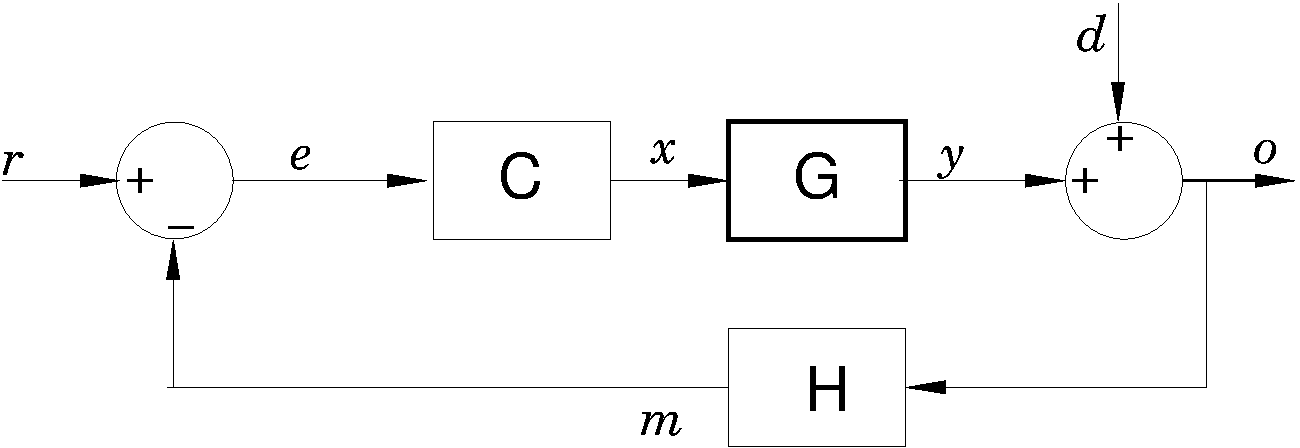
\includegraphics[scale=0.7]{feedback-loop-3.pdf}
	\caption{Dinâmica e comportamento da chaleira aquecendo}
	\label{fig:feedback-nobile}	
	\fdireta{Nobile2013}
\end{figure}

O projeto de \cite{Nobile2013} foi ao encontro de soluções adaptativas para gerenciamento de recursos e disponibilização de aplicações na computação em nuvem. O trabalho optou por aplicar técnicas de adaptação ainda pouco exploradas nas Computação, mas de reconhecimento há décadas por outros áreas da ciência e engenharia. A técnica utilizada foi a teoria de controle, que conta como uma rica coleção de ferramentas de linguagem matemática. Ferramental que auxiliam na descrição do comportamento de sistemas dinâmicos em termos de como eles respondem a diferentes estímulos em regime estacionário e transiente.

Talvez uma das primeiras definições de um sistema dinâmico foi feito por \cite{tsonis1989} , que definiu como:
\begin{citacao}
	Em termos simples, é um sistema cuja evolução a partir de um estado inicial pode ser descrito por alguma regra(s). Estas regras são convenientemente expressas como equações matemáticas. A evolução de um tal sistema é melhor descrito pelo chamado espaço de estado.
\end{citacao}

Já a definição de \cite{willems2013} diz que o adjetivo dinâmico refere-se aos fenômenos com uma reação retardada, fenômenos com um efeito colateral, com transientes, oscilações, e, talvez, uma abordagem para o equilíbrio. Em suma, os fenômenos em questão é a evolução no tempo. Vemos um sistema dinâmico no contexto lógico de definição simples como um modelo matemático, mas um modelo matemático em que os objetos de interesse são funções do tempo: o universo é um espaço de funções. Tomamos o ponto de ver que um sistema dinâmico constrange os sinais do tempo que o sistema pode conseguir produzir.

Sistemas dinâmicos são objetos matemáticos usados para modelar fenômenos físicos cujo estado ou descrição instantânea muda com o tempo. Estes modelos são utilizados na previsão econômica e financeira, modelagem ambiental, diagnóstico médico, o diagnostico equipamento industrial, e uma série de outras aplicações \cite{Dean1991}.

Para \cite{Scheinerman1995} a dificuldade é que qualquer coisa que evolui ao longo do tempo pode ser considerado um sistema dinâmico. Em seu livro, \cite{Scheinerman1995}, inicia descrevendo sistemas dinâmicos matemáticos, mas para o autor um sistema dinâmico tem duas partes: um vetor de estado que descreve exatamente o estado de algum sistema real ou hipotético, e uma função (ou seja, uma regra) que nos diz, dado o estado atual, o que o estado do sistema será no próximo instante de tempo.

É claro que é possível representar sistemas físicos (e.g. eletrônicos, químicos e biológicos), mas para fins didáticos e em geral, é comum utilizar de sistemas mecânicos e eventos rotineiros para exemplificar a dinâmica dos sistemas:

\begin{description}
	\item[Uma chaleira em aquecimento:] Imagine uma chaleira com água em um fogão convencional em contato a uma chama (tudo sob condições normais de temperatura e pressão), a água presente dentro da chaleira não saltará imediatamente para a temperatura final da chama, pelo contrário, a água do recipiente mostra um aquecimento gradual. O mesmo ocorrerá, mas de maneira inversa, quando a chama do fogo for apagada, a temperatura da água não sofrerá uma queda brusca imediatamente mas, lentamente diminuirá até a temperatura ambiente.
	
	\begin{figure}[htb]
		\centering
		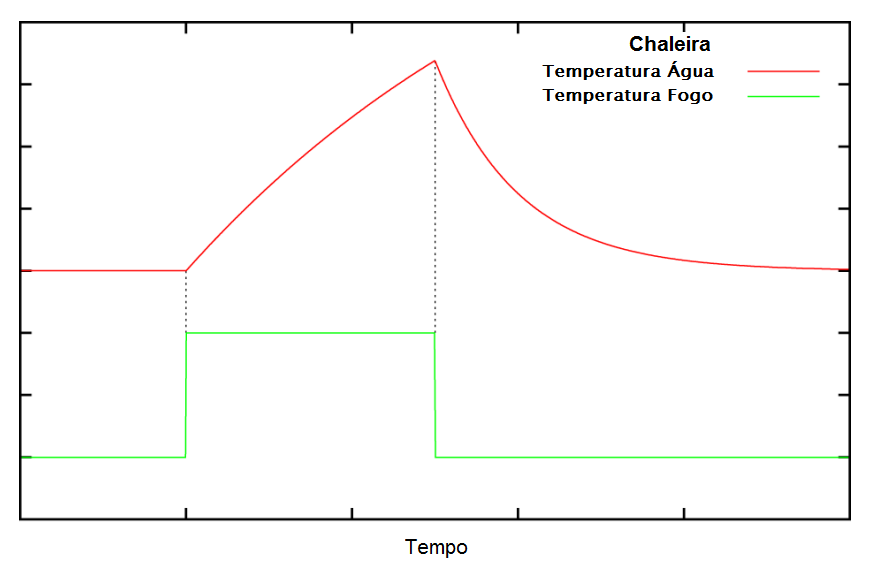
\includegraphics[scale=0.5]{grafico-chaleira.png}
		\caption{Dinâmica e comportamento da chaleira aquecendo}
		\label{fig:chaleira}
		\fdireta{Janert2013}
	\end{figure}
	
	Neste caso da chaleira em aquecimento, o aumento e a constante temperatura da chama (enquanto o fogo ligado, fornecendo calor) representa a entra do sistema, como indicado pela linha verde da figura \ref{fig:chaleira}, e o aquecimento da água representa o comportamento do sistema mediante a entrada, conforme demonstrado pela linha vermelha da figura \ref{fig:chaleira}. 
	
	\item[Uma massa em uma mola:] Agora considere uma massa, em repouso, suspensa por uma mola, também em repouso e fixa em uma superfície plana. Ao deslocarmos o peso tirando-o do repouso e soltarmos após o tencionamento da mola, a massa iniciará uma oscilação até o instante em que a massa e a mola voltarem ao equilíbrio inicial.	
	
	\begin{figure}[!htb]
		\centering
		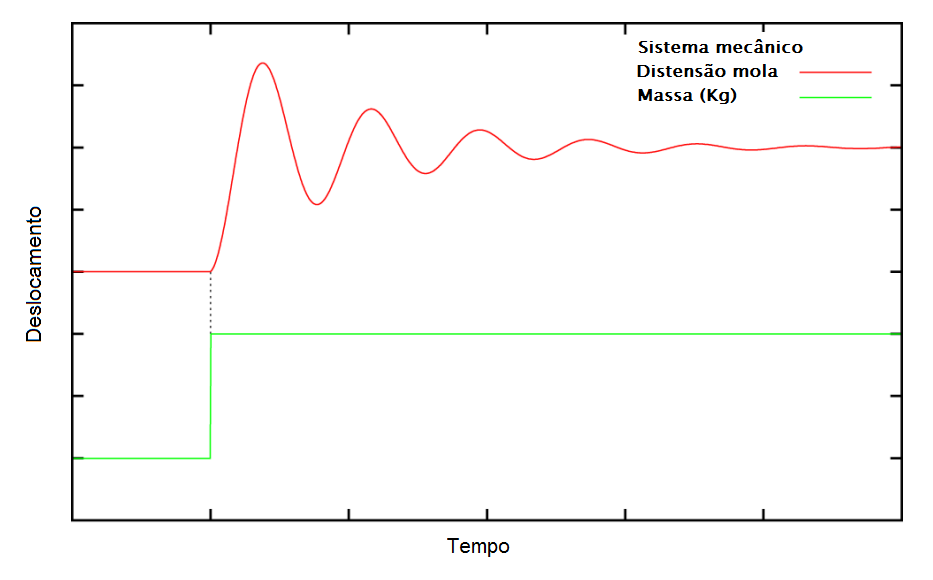
\includegraphics[scale=0.5]{grafico-mola.png}
		\caption{Dinâmica e comportamento da mola}
		\label{fig:mola}		
		\fdireta{Janert2013}
	\end{figure}
	
	O deslocamento inicial (entrada do sistema), por nós provocados, é representado pela linha verde na figura \ref{fig:mola} e a oscilação subsequente em resposta à força aplicada é representado pela linha vermelha no mesma figura \ref{fig:mola}.
\end{description}

Os exemplos de sistemas dinâmicos, apresentados acima, e as suas respostas aos estímulos externos, são comportamento comuns em sistemas computacionais e estes aspectos são negligenciados em muitos sistemas, pois até então os sistemas computacionais tem-se comportado com uma dinâmica imperceptível aos usuários. Entretanto, os atuais sistemas computacionais tem tomado tamanha proporção que já não tem respondido imediatamente a uma oscilação na carga de entrada, apresentando características de dinâmica \cite{Janert2013}, como demonstrado pelo trabalho de \cite{Nobile2013}, que demonstra que as características dinâmicas de um ambiente de computação em nuvem de larga escala tem impacto apreciável no desempenho dos mecanismos de provisão de QoS.


Embora a análise transiente ainda seja pouco explorada frente as principais abordagens de avaliação de desempenho, em outra obra cientifica do LaDSPC é a \cite{Lourenco2015} que abrange sobre o tema e sua importância para sistemas computacionais. A abordagem predominante à avaliação de desempenho dos sistemas computacionais considera na análise da capacidade no estado estacionário. Geralmente se deseja descartar efeitos de inicialização e, em seguida medir o desempenho quando a saída se estabilizou. A razão para a proeminência na análise estacionária é devido a não importância da dinâmica em sistemas computacionais tradicionais. Normalmente, as plataformas de computador respondem suficientemente rápido as alterações operacionais que afetem o desempenho. Estas justificativas, no entanto, não assegura necessariamente para sistemas distribuídos emergente, especialmente em ambientes de grande escala e aplicações de vários níveis. O efeito de pequenos atrasos e a propagação para outras camadas podem render comportamento dinâmico significativos \cite{Lourenco2015}.

Durante o regime transitório, o desempenho pode apresentar comportamentos diferentes, dependendo da dinâmica do sistema: ele pode variar abruptamente, ou lenta e progressivamente, e até mesmo presentes componentes oscilatórios. Análise em regime transitório pode revelar capacidade dinâmica do sistema dependendo das suas propriedades inerciais \cite{Lourenco2015}.

Segundo \cite{Janert2013}, a resposta de um sistema a uma perturbação externa muitas vezes consiste em um componente transiente, que desaparece ao longo do tempo, e um componente de estado estacionário. Como demonstrados anteriormente, os componentes diluem no decorrer do tempo, caracterizando-os como transitórios. 

Este conjunto de exemplos tem por objetivo mostrar a importância da avaliação de desempenho principalmente quando um sistema se encontra no regime transiente, pois podem influenciar diretamente no desempenho do sistema. Na avaliação de desempenho de sistemas computacionais é muito comum a irrelevância e o desprezo quando um sistema apresenta \newword{\textit{warm-up}}{período em que o sistema se encontra em regime transiente} principalmente quando a avaliação se concentra em analisar o regime estacionário do sistema. Sendo assim, medidas de interesse de regime transientes, como a amplitude máxima atingida pela resposta do sistema e o tempo de assentamento ou ajuste são interessantes para que se possa medir e analisar o comportamento do sistema \cite{Nobile2013}.

No trabalho de \cite{Lourenco2015}, o artigo discute sobre a abordagem de análise de estado estacionário vigente para avaliação de desempenho de sistemas computacionais e apresenta uma abordagem para o planejamento de experimentos de simulação destinados a análise transitória, especialmente em aplicações \textit{multi-tiers}.
O trabalho de \cite{Lourenco2015} inicia discutindo sobre as propriedades dinâmicas de sistemas computacional de grande escala em ambientes distribuídos e como estas características podem afetar o desempenho. As dinâmicas emergentes da interligação de sistemas computacionais de \textit{multi-tiers} e escaláveis, podem produzir efeitos transitórios sobre o desempenho, como resposta temporal e comportamento oscilatório, sendo que estes efeitos variáveis no tempo pode afetar a capacidade de resposta, eficiência e até mesmo a estabilidade do mesmo. 

\begin{citacao}
	Nesse contexto, técnicas de identificação de sistema, análise dinâmica, refere-se à estrutura matemática utilizada para identificar e representam as propriedades dinâmicas de sistemas que apresentam um comportamento inercial, tais como reação e oscilatório amortecido \cite{Lourenco2015}. 
\end{citacao}

Embora a avaliação de desempenho em sistemas computacionais se estabeleceu como um campo de pesquisa nas últimas décadas, esta não se adequa para sistemas dinâmicos, em geral à avaliação de desempenho de sistemas computacionais considera análise da capacidade em estado estacionário onde se descarta os efeitos de inicialização e, em seguida mede o desempenho quando a saída já se estabilizou. Em um cenário comum, em que a avaliação necessita responder a perguntas como, \textit{Qual a quantidade de carga de trabalho pode a alça do sistema antes de degradar excessivamente ?}, ou como, \textit{Qual o é o desempenho do sistema com uma determinada carga de trabalho ?}, para uma estimativa quantitativa, este experimento é suficiente para expor o sistema \cite{Lourenco2015}.
Como pode-se entender, a análise estacionária na avaliação de desempenho em sistemas computacionais é devido a não importância da dinâmica no sistema. Normalmente, os sistemas são suficientemente rápido responder a alterações que afetam o desempenho. Especialmente em ambientes computacionais de grande escala e aplicações de \textit{multi-tiers}, o efeito de pequenos atrasos e propagação para com muitos subsistemas interligados pode render comportamento dinâmico significativa, apreciáveis como efeitos inerciais na resolução de tempo de resposta. 

Durante os períodos descartados na avaliação estacionaria, o chamando regime transitório, o desempenho pode apresentar comportamentos diferentes, dependendo da dinâmica do sistema, variando abruptamente, lentamente, ou até mesmo presentes comportamentos oscilatórios. Contrastando a identificação do sistema de estado estacionário, um modelo analítico deste tipo prevê o desempenho em função da carga de trabalho e tempo.

Ainda no mesmo trabalho, \cite{Lourenco2015} apresenta um conjunto de requisito que especificam uma arquitetura conceitual, intitulada \textit{\sigla{MEDC}{\textit{Monitor, Effector, Demanda and Capacity}}} representado pela figura \ref{fig:extension-block}. O diagrama ilustra a arquitetura que tem quatro preocupações essenciais: \textit{Demand}, \textit{Capacity}, \textit{Monitor} and \textit{Effector}.

\begin{description}
	\item[\textit{Demand}:] é uma referência para a capacidade de modulação e deve ser configurada de modo a especificar a forma como a carga de trabalho muda ao longo do tempo,
	\item[\textit{Capacity}:]  é a disposição análoga no que diz respeito aos recursos do sistema,
	\item[\textit{Monitor}:] desempenha o papel de um sensor e aquisição de dados temporais, sendo seu dever de coletar os dados sobre o sistema e torná-lo disponível,
	\item[\textit{Effector}:] representam os mecanismos de atuação através modulação da capacidade, que serve como uma camada de abstração disponível para a modelagem dos componentes operacionais que afetam a dinâmica \textit{Capacity} e \textit{Demand};
\end{description}

\begin{figure}[!htb]
	\centering
	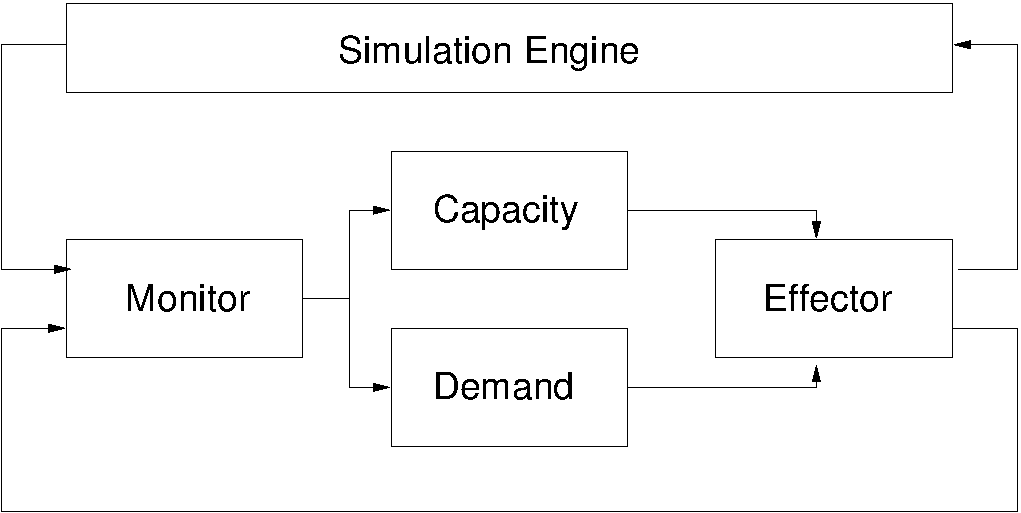
\includegraphics[scale=0.8]{extension-block.pdf}
	\caption{Arquitetura conceitual MEDC}
	\label{fig:extension-block}
	\fdireta{Lourenco2015}
\end{figure}

O fluxo de trabalho, esta associada a responsabilidade de controlar a geração de carga com os ciclos de simulação e, correspondentemente, no que diz respeito à capacidade. Este controle se traduz em uma política de tomada de decisão que acionar eventos que solicitam a criação ou o despedimento de novas entidades de carga de trabalho e de recursos. A ordem é efetivamente realizado pelo \textit{Effector}, que recebe as solicitações dos controladores de \textit{Demand} e \textit{Capacity} e os manipula antes de transmitir os eventos para o mecanismo de núcleo. É através do \textit{Capacity} que pode-se modelar, por exemplo, atrasos associados a alocação e deslocação, de políticas de escalonamento, enchimento do \textit{buffers}, os tempos de resposta do hardware, padrões de falha de recurso, etc. O dever do \textit{Monitor} está em alimentar a \textit{Demand} e a \textit{Capacity} de dados sobre qualquer estado, por exemplo, utilização média do sistema, tempo de permanência trabalho, relação de perder \textit{deadline}, etc. Para cada um dos quatro responsabilidades, a uma ação e é associado de forma iterativa em cada etapa do ciclo de simulação \cite{Lourenco2015}. 

\begin{figure}[!htb]
	\centering
	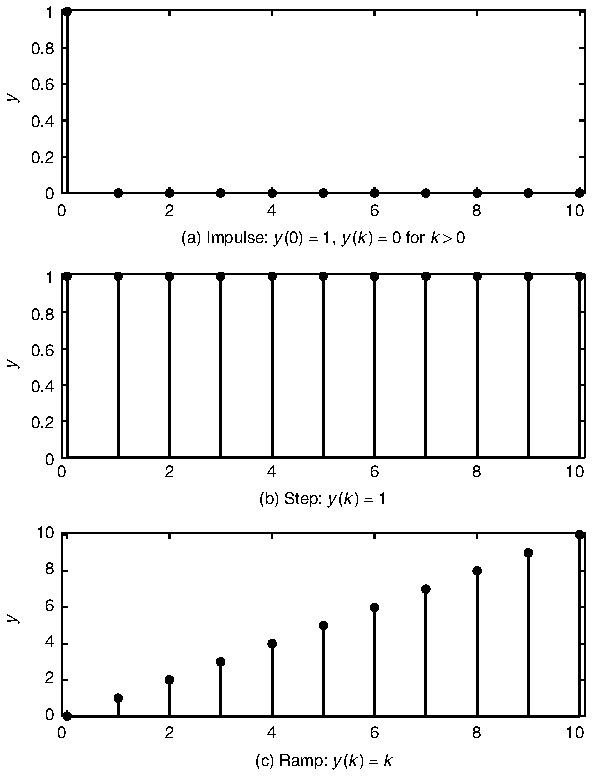
\includegraphics[scale=1.2]{funcoes1.pdf}
	\caption{Sinais em tempo discreto comuns, parte 1}
	\label{fig:funcoes1}
	\fdireta{Hellerstein2004}
\end{figure}

A fim de trazer essas propriedades dinâmicas, a experiência de simulação deve excitar o sistema com carga de trabalho não-estacionária sob condições controladas. Para que seja possível apreciar e apresentar a dinâmica de um sistema e realizar a análise transitória do sistema, é preciso utilizar cargas de trabalho que possam provocar comportamentos propícios, onde as caraterísticas dinâmicas do sistema sejam claramente observadas, em \cite{Hellerstein2004}, apresenta propostas de algumas funções, ou sinais, de perturbação, por exemplo: impulso, degrau, rampa, seno, exponencial, seno modulada por uma exponencial, etc.  Essas funções são apresentadas nas figuras \ref{fig:funcoes1} e \ref{fig:funcoes2}.

\begin{figure}[!htb]
	\centering
	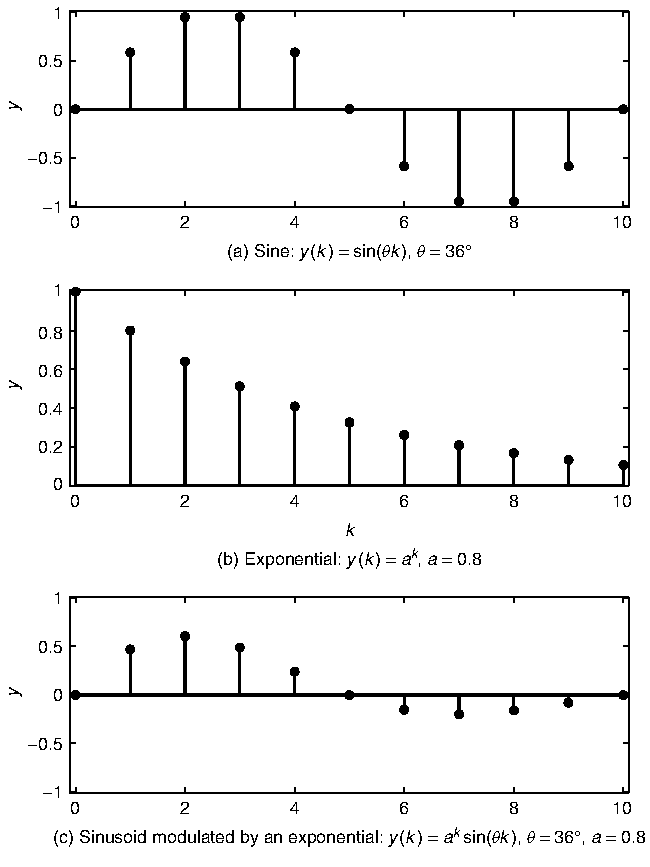
\includegraphics[scale=1.2]{funcoes2.pdf}
	\caption{Sinais em tempo discreto comuns, parte 2}
	\label{fig:funcoes2}
	\fdireta{Hellerstein2004}
\end{figure}

Para a geração de carga para sistemas existem outras propostas que permitem simular um comportamento mais realística \cite{Mi2010, Mi2009,Mi2008}. Mais especificamente, em \cite{Menasce2002}, é apresentada uma outra metodologia para geração de cargas de trabalho que emulam o fenômeno aumento temporal em uma forma controlável. Por exemplo, é de grande interesse fornecer um mecanismo que permite o teste e avaliação do desempenho do sistema sob cargas de trabalho do tipo rajadas. Esta nova metodologia permite injetar quantidades diferentes de rajada dentro do fluxo de chegada utilizando o índice de dispersão. 

Nesse contexto Choquehuanca, pretende utilizar a especificação de arquitetura proposta por \cite{Lourenco2015} em um ambiente real. Este trabalho irá atuar diretamente no requisito \textit{Demand} da arquitetura conceitual MEDC, este requisito será implementado em um benchmark definido por Choquehuanca.

\textit{Benchmarking} é o principal método para medir o desempenho de uma máquina ou sistema. O \textit{benchmarking} refere-se à execução de um conjunto de programas representativos em diferentes computadores e redes, medindo os resultados. Esses resultados são utilizados para avaliar o desempenho de um determinado sistema com uma carga de trabalho bem definida \cite{Menasce2001}.

O \textit{benchmarking} pode ser visto como um modelo de identificação de oportunidades com o intuito de aumentar a competitividade em ambientes gradativamente turbulentos, assim teve seu surgimento a partir da década de 70 e, tornou-se importante devido às falhas dos métodos tradicionais de fixação de metas que algumas empresas americanas adotavam para enfrentar a concorrência externa, principalmente pelos produtos japoneses \cite{Camila2008}. Para \cite{Marco2012} \textit{benchmarks} são um padrão de ferramentas que permitem avaliar e comparar diferentes sistemas ou componentes de acordo com características especificas, tais como desempenho, confiabilidade e segurança. Segundo \cite{Folkerts2013} \textit{benchmarks} são ferramentas para responder a uma pergunta \textit{"Qual é o melhor sistema em um determinado domínio?"} ou  \textit{"Qual é o melhor processador?"} ou ainda responde à pergunta \textit{"Qual é o melhor sistema de banco de dados para OLTP?"}. Para \cite{Folkerts2013}, a interpretação concreta do \textit{"qual o melhor"} depende do objetivo do \textit{benchmarking}, e esta deve ser a primeira pergunta a ser respondida na concepção de um novo \textit{benchmark}. 


Segundo \cite{Stefan2010} a definição de um \textit{benchmarking} é o ato de medir e avaliar o desempenho computacional, sob condições de referência e em relação a uma avaliação de referência. O objetivo do \textit{benchmarking} é permitir a comparação equitativa por diferentes soluções, ou entre desenvolvimentos subsequentes de um sistema em teste (\sigla{SUT}{System Under Test}). Estas medidas incluem métricas principais de desempenho caracterizando o ambiente em que o SUT está hospedado.

A \textit{Xerox Corporation} é geralmente creditado com o início dos primeiros projetos de avaliação de desempenho global, em 1979. Alertado por uma suspeita de que os custos de produção de máquinas fotocopiadoras foram significativamente mais elevados nos EUA do que no Japão, estas iniciativas \textit{benchmarking} foram utilizados pela Xerox para obter direitos quanto aos materiais, processos e métodos utilizados pelos japoneses. Uma aplicação das lições aprendidas através de \textit{benchmarking} permitiu a \textit{Xerox} aumentar a eficiência de design e produção, e, consequentemente, para reduzir os custos de fabricação de suas máquinas fotocopiadoras. Isto não só reforça a posição de competitiva da \textit{Xerox} no mercado, mas também levou ao desenvolvimento e evolução de uma nova ferramenta gerencial, conhecido como processo de \textit{benchmarking} \cite{Mahmoud2002}.

No contexto de sistemas de simulação, \textit{benchmark} é um software capaz de gerar carga de trabalho a ser aplicada a um sistema computacional com o objetivo de gerar dados acerca de uma métrica de forma que seja possível medir e comparar o desempenho de sistemas sob observação. Para os fabricantes de novos produtos, um \textit{benchmark} pode fornecer informações estatísticas importantes para que eles possam ser ajustados antes da sua implantação. Por outro lado, para os usuários finais, permite ter um ponto de referência na comparação entre pontos fortes e fracos de diferentes produtos. \textit{Benchmarks} ajudam em estimativas de escalabilidade em termos do número de usuários e/ou operações que um sistema pode suportar, e os tempos de resposta do sistema sob várias cargas e plataformas de implantação em hardware/software \cite{Jutla1999}.

O desenvolvimento de um bom \textit{benchmark} tem sido considerada uma "arte negra" por um longo tempo, devido a inumaras sutilezas que influenciam o sucesso do \textit{benchmark}. 
No entanto, pesquisas e estudos com base em \textit{benchmarks} para sistemas computacionais não é um tema novo, para explorar o caminho que levará à uma boa metodologia de extensão, começamos por rever as propriedades pertinentes de um \textit{benchmarks}, assim a metodologia incorporará dessas boas práticas para o objetivo de extensão.
As definições de um \textit{benchmark} são temas para uma série de trabalhos que tentam fornecer orientações sobre o assunto, as investigações relacionadas sugerem uma série de orientações amplamente aceitas e critérios de qualidade que devem ser considerados no projeto e execução de \textit{benchmark}, como os trabalhos publicados \cite{Kistowski2015, Chen2014, Folkerts2013, Marco2012, Huppler2009, Gray1992} que tem identificado as seguintes características:


\begin{description}
	\item[Relevância] é, talvez, a característica mais importante de um \textit{benchmark}. Mesmo que a carga de trabalho for perfeita em todos os outros aspectos, será de uso mínimo se ele não fornece informações relevantes para seus usuários. No entanto, a relevância é também uma característica de como os resultados do \textit{benchmark} são aplicadas; \textit{benchmarks} pode ser altamente relevante para alguns cenários e ter mínima relevância para outros, para o usuário do \textit{benchmark}, uma avaliação da relevância de um ponto de referência deve ser feita no contexto da utilização prevista desses resultados para o \textit{benchmark} \cite{Kistowski2015}. 
	
	\item[Reprodutibilidade] a capacidade de produzir os mesmos resultados de forma consistente para um ambiente de teste em particular, inclui a consistência e capacidade para um outro testador reproduzir de forma independente os resultados em outro sistema. A capacidade de reproduzir os resultados em outro ambiente de teste é em grande parte ligada à capacidade de construir um ambiente equivalente. \textit{Benchmarks} de indústria requer além de resultados uma descrição do ambiente de teste, geralmente incluindo hardware e componentes de software, bem como opções de configuração, da mesma forma que a pesquisa publicada, que inclui resultados de \textit{benchmark} geralmente inclui uma descrição do ambiente de teste que produziu esses resultados. No entanto, em ambos os casos, a descrição não pode fornecer detalhes suficientes para um laboratório independente para ser capaz de montar um ambiente equivalente. \textit{Hardware} deve ser descrito o suficiente em detalhe para uma outra pessoa possa obter um idêntico. As versões de \textit{software} deve ser indicado de modo que seja possível usar as mesmas versões ao reproduzir o resultado. Opções de ajuste e configuração devem ser documentadas para versão de \textit{firmware}, sistema operacional e aplicativo de \textit{software} para que as mesmas opções podem ser usadas quando reexecutar o teste. \cite{Kistowski2015}
	
	\item[Verificabilidade] Dentro da indústria, \textit{benchmarks} são normalmente executados por fornecedores que têm interesse nos resultados. Na academia, os resultados são submetidos a revisão por pares e resultados interessantes será repetido e desenvolvido por outros pesquisadores. Em ambos os casos, é importante que os resultados do \textit{benchmark} são verificáveis, de modo que os resultados podem ser considerados dignos de confiança. \cite{Kistowski2015}
	
	\item[Usabilidade] A maioria dos usuários de \textit{benchmarks} são normalmente técnicos, tornando a facilidade de uso uma preocupação menor do que é para aplicações pensadas e desenvolvidas para o consumidor. Existem, no entanto, várias razões por que a facilidade de utilização seja importante.
	Isso já foi discutido em termos de fazer \textit{benchmark} verificável. Outro aspecto da facilidade de utilização é ser capaz de construir configurações práticas para a execução do \textit{benchmark}. Descrições precisas sobre o hardware do sistema e software configuração são críticas para a reprodutibilidade, mas pode ser um desafio, devido à complexidade dessas descrições.
	\textit{Benchmarks} pode melhorar a facilidade de utilização, fornecendo ferramentas para ajudar com este processo. \cite{Kistowski2015}
	
	\item[Escalável] deve ser apoiada em uma maneira que preserve a relação com o cenário de negócios próximo ao modelo real. Além disso, o usuário deve ser oferecida a possibilidade de dimensionar a carga de trabalho de forma arbitrária pela definição de um conjunto próprio de pontos de escala. \cite{Marco2012}
	
	\item[Simplicidade] Os elementos conceituais de \textit{benchmark} deve ser reduzida ao mínimo e feito facilmente compreensível. O \textit{benchmark} também deve abstrair detalhes que representam configurações de caso a caso, ou escolhas de administração do sistema e não afetam o desempenho. \cite{Chen2014} Um \textit{benchmark} com uma estrutura altamente complexa é muitas vezes difícil de entender e difícil confiar. Se as pessoas não confiam no \textit{benchmark}, elas não vão usá-lo. \textit{Benchmarks} deve, portanto, ser o mais simples possível. Complexidade necessária pode ser explicado em uma documentação do \textit{benchmark} \cite{Weber2014}.
	
	\item[Econômico] Ele é muitas vezes negligenciado durante o desenvolvimento inicial do \textit{benchmark}, pois as fases iniciais do desenvolvimento estão focados em imitar a realidade para fornecer a relevância necessária para o \textit{benchmark}. Na verdade, para ser relevante, pode-se esperar uma \textit{benchmark} realista; e ser realista, muitas vezes significa ser complexo; e complexo para ser invariavelmente significa ser caro. Esta é claramente uma outra oportunidade para o compromisso, se alguém quiser criar uma \textit{benchmark} de sucesso. O termo "econômico", não significa "barato", mas sim "vale o investimento".
	Considere os resultados da IBM, TPC-C ou TPC-E ou TPC-H e alguns da SPEC, SPECjAppServer2004 e  SPECweb2005, todos eles selecionam apenas uma fatia da "realidade total" da indústria da informática, no retorno para o apelo de ser barato para correr, fácil de executar e fácil de verificar. Enquanto eles não são usados fora do contexto da sua intenção, eles também atendem aos requisitos para a relevância, equidade e repetibilidade. \cite{Huppler2009}
	
	\item[Métrica] uma métrica significativa ser compreensível e é obrigado a relatar sobre as reações do SUT referentes à carga. \cite{Folkerts2013} as métricas do \textit{benchmark} deve permitir caracterizar e quantificar o comportamento do sistema quando enfrenta perturbações (ou seja, falhas, ataques, e variações de ambiente operacional). À vista primeiro, resiliência métricas de \textit{benchmark} deve caracterizar o desempenho, confiabilidade e segurança \cite{Marco2012}.
	
\end{description}

Nas abordagens mencionadas acima, referente as propriedades de um \textit{benchmarks} de sucesso, segundo os autores, e nenhum dos trabalhos contemplam uma metodologia de extensão em que o \textit{benchmark} pode ser desenvolvido. Na seção em sequência, este trabalho propõe tal metodologia, e nos capítulos seguintes foi ilustrado atrás vez de um caso de estudo a extensão de um \textit{benchmark} usando tal metodologia. É importante compreender as características de uma carga de trabalho e determinar se ou não é aplicável para uma situação particular. Ao desenvolver uma nova carga de trabalho, as metas devem ser definidas para que escolhas entre os critérios de projeto concorrente pode ser feita de acordo com esses objetivos para alcançar o equilíbrio desejado. \cite{Kistowski2015}

Antes de definir a metodologia propriamente dita, é importante assegurar que não é qualquer \textit{benchmarks} que pode ser modificado pela extensão, existe alguns pré-requisitos e estes são apresentados. No trabalho \cite{Folkerts2013} apresenta a definição de três grupos de requisitos, com base nas propriedades apresentadas anteriormente:

\begin{description}
	\item[1. Requisitos gerais] - este grupo contém requisitos genéricos. 
	\begin{itemize}
		\item Relevância
		\item Econômico
		\item Simplicidade
	\end{itemize}
	
	\item[2. Requisitos de Implementação] - este grupo contém as exigências relativas à implementação e desafios técnicos. \hfill 
	\begin{itemize}
		\item Fair e portáteis
		\item Reprodutibilidade
		\item Realista
		\item Relevância
	\end{itemize}
	
	\item[3. Requisitos de Carga de Trabalho ] - contém os requisitos quanto à definição de carga de trabalho e suas interações. \hfill 
	\begin{itemize}
		\item Representatividade
		\item Escalável
		\item Métricas
	\end{itemize}
	
\end{description}


\textit{E-commerce}, que é uma loja virtual de comercio eletrônico, tem se tornado cada vez mais popular e ganhado cada vez mais concorrência com o desenvolvimento e expansão da Internet.O Bench4Q é um \textit{benchmarking} que segue a metodologia de \textit{e-commerce} orientado a QoS, providos de recursos que permitem a simulação de um ambiente controlavel e flexível. Além disso, o Bench4Q pode ser usado para avaliar o desempenho de escalabilidade do sistema.

O trabalho \cite{cherkasova1998}, apresenta o conceito de sessão, que define uma sequencia de requisições de um único cliente. \cite{Krishnamurthy2006}, apresenta a dependência de sessões em sistemas \textit{e-commerce} e ressalta a importância de caracterizar a carga de trabalho sintética.

Apesar do grande sucesso do \sigla{TPC-W}{\textit{Transaction Processing Performance Council - Web}} \footnote{TPC-W: \url{http://www.tpc.org/tpcw/}}, existe diversos trabalhos que apresentam métricas baseadas em sessões mais úteis do quais utilizadas pelo \textit{benchmark}. Ainda assim existe outro conjunto de trabalhos concentrado em como fazer TPC-W ser mais realístico. Em geral, essa obras tem inserido \textit{burstiness} na simulação de carga. O trabalho \cite{Mi2009} de Casale, incluiu o comportamento de \textit{burstiness}. Enquanto a obra \cite{Sobel2008}, busca adaptar o TPC-W para o ambiente em nuvem.

Embora a grande diversidade dos trabalhos apresentados, o Bench4Q oferece uma solução integrada para \textit{e-commerce} sensíveis a QoS. Vale salientar que, não há nenhuma solução integrada as características, especialmente, a de encontrar qualquer extensão TPC-W sensível a QoS para \textit{e-commerce}. Contudo, existem trabalhos que abordam a modelagem de rajadas no processo de chegada da carga de trabalho imposta ao sistema \textit{e-commerce}. \cite{Casale2012}, apresenta o \sigla{BURN}{\textit{BURtiness eNabling method}}, uma metodologia para gerar rajadas customizáveis como demanda de carga de trabalho afim de avaliar o desempenho de um sistemas \textit{e-commerce}. A metodologia BURN é composta de duas políticas tradicional (que gera a carga de trabalho constante a mesma gerada pelo TPC-W) e a \textit{burst} (que insere as rajadas na carga de trabalho tradicional). Durante a execução do \textit{benchmark}, BURN aplica um stress na aplicação \textit{e-commerce} alternando as duas políticas. Tais trabalhos buscam avaliar o desempenho sistemas de multi-camadas (composto por um servidor de aplicação, base de dados, etc) que hospedem um \textit{e-commerce} como é o caso do Bench4Q.


Sistemas de \textit{e-commerce} tem uma grande preocupação com os níveis de QoS, pois estão relacionados diretamente com os lucros do website. Atualmente a maioria dos \textit{e-commerce} são desenvolvido sensível a QoS. O Bench4Q é um \textit{benchmark} de um \textit{e-commerce} sensível a QoS.  Com o desenvolvimento da tecnologia Web, o TPC-W se tornou uma referência de \textit{e-commerce}, entretanto a implementação do TPC-W é insuficiente para \textit{e-commerce} sensíveis a QoS.

A maioria dos \textit{benchamarks} de \textit{e-commerce}, incluindo o TPC-W, são limitados para os sistemas sensíveis a QoS. As métricas utilizadas são baseadas em requisições \sigla{HTTP}{\textit{Hypertext Transfer Protocol}}, como a taxa de requisições atendidas com sucesso ou o tempo de resposta das requisições. Embora uma das características mais críticas de um sistema de \textit{e-commerce} sensíveis a QoS seja a integralidade do serviço prestado aos clientes, as métricas baseada em requisições podem levar a afirmações ineficientes e até mesmo erradas.

O Bench4q é uma extensão do TPC-W \cite{Menasce2002}, e tem como objetivo o \textit{tuning} de servidores \textit{e-commerce} orientados a fornecer QoS aos seus clientes. As principais características do Bench4Q incluem: 
Apoio à análise de métricas baseada em sessão que simula carga sensível a QoS para uma análise da capacidade. 

O \textit{benchmark} Bench4Q, é distribuído de acordo com a \sigla{GNU}{\textit{ Lesser General Public License}}, sendo um software livre ele pode ser redistribuído e/ou modificado sob os termos da licença publicas pela \textit{Free Software Foundation}. Seguindo muitas diretrizes da especificação TPC-W, o Bench4Q usa principalmente nas suas métricas de simulação de carga e garantia de QoS \cite{Bench4Q}. 

O Bench4Q oferece uma arquitetura distribuída para a geração de carga através de seus agentes que são conectados a um único console que os gerencia, entretanto é possível configurar separadamente as configurações para cada agente. Esses agentes geram carga (requisições HTTP) para o servidor de aplicação onde esta hospedado o \textit{e-commerce} como ilustrado na figura \ref{fig:arquitetura-bench4q}. Os resultados da avaliação de carga aplicada ao \textit{e-commerce} são coletados pelo console que apresenta alguns gráficos, que facilita a interpretação da avaliação mediante as diretrizes do TPC-W que são complexas \cite{Bench4Q}.

A ferramenta é composta por três partes: Console, Agente e SUT, conforme apresenta a figura \ref{fig:arquitetura-bench4q}, e também disponibiliza interfaces para o monitoramento de recursos para o servidor de aplicação e para o banco de dados, este monitoramento incluem CPU, memória, rede, etc.


\begin{figure}[htb]
	\centering
	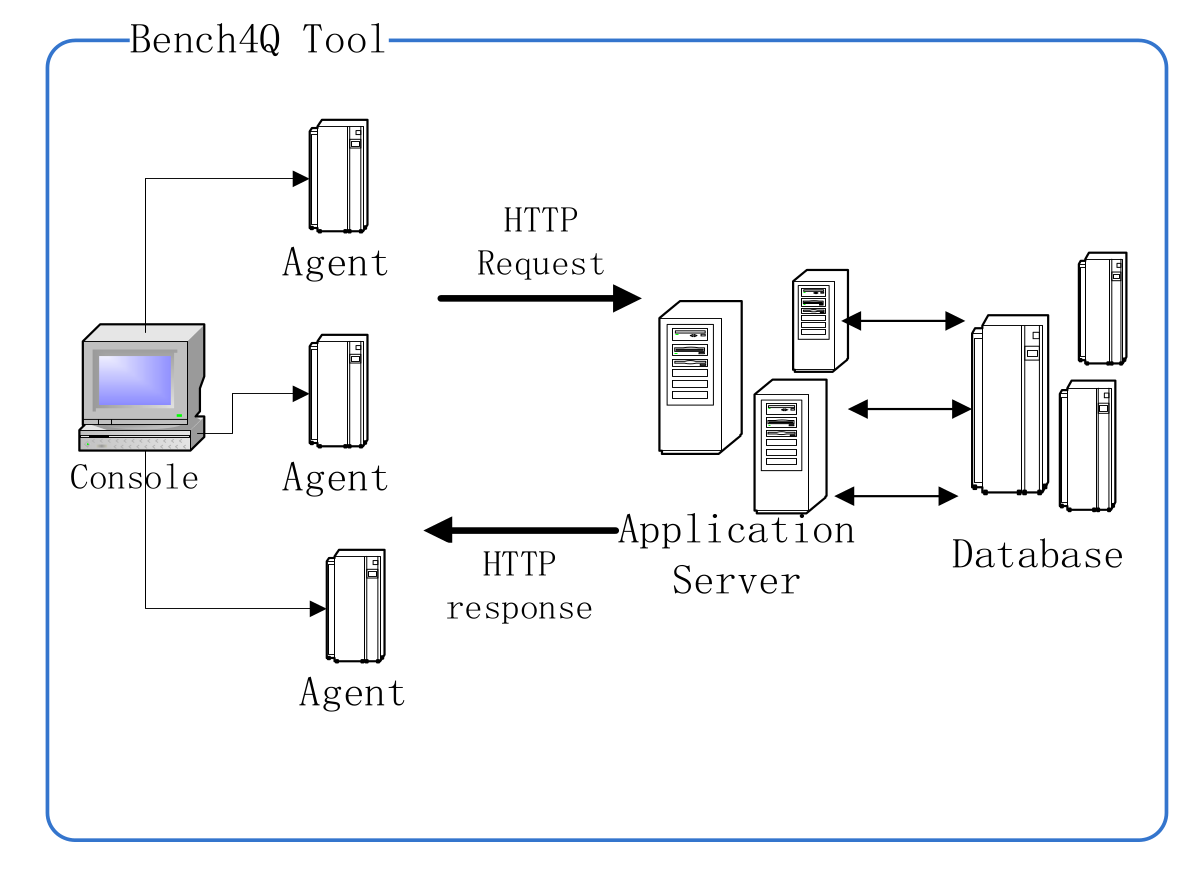
\includegraphics[scale=0.3]{bench4Q.png}
	\caption{Arquitetura Bench4Q}
	\label{fig:arquitetura-bench4q}
	\fdireta{Bench4Q}
\end{figure}

\begin{itemize}
	
	\item \textbf{Console:} A figura \ref{fig:console-bench4q} apresenta a interface do console, onde configura-se o teste, coleta e exibe os resultados. 
	
	\begin{figure}[!htb]
		\centering
		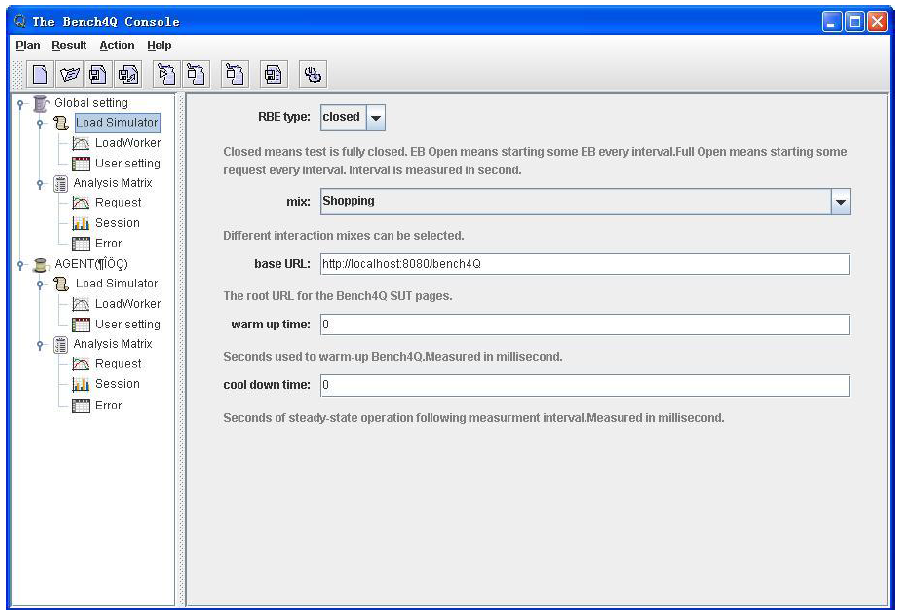
\includegraphics[scale=0.7]{console-bench4Q.png}
		\caption{Console Bench4Q}
		\label{fig:console-bench4q}
		\fdireta{Bench4Q}	
	\end{figure}
	
	\item \textbf{Agente:} É este que faz o trabalho real, pois gera a carga configura no console. Simula o comportamento dos usuários no \textit{website}, disparando diversas requisições para o \textit{e-commerce}. 
	
	\item \textbf{SUT:} O \textit{e-commerce} SUT (\textit{System Under Test}), conforme apresentado na figura \ref{fig:sut},  é quem fornece o website de compras e está organizado com um banco de dados, servidor web e servidor de aplicativos. O portal compreende todos os componentes que fazem parte de uma aplicação real, isso inclui as conexões de rede, servidores web, servidores de aplicação, servidores de banco de dados, etc.
	
	\begin{figure}[htb]
		\centering
		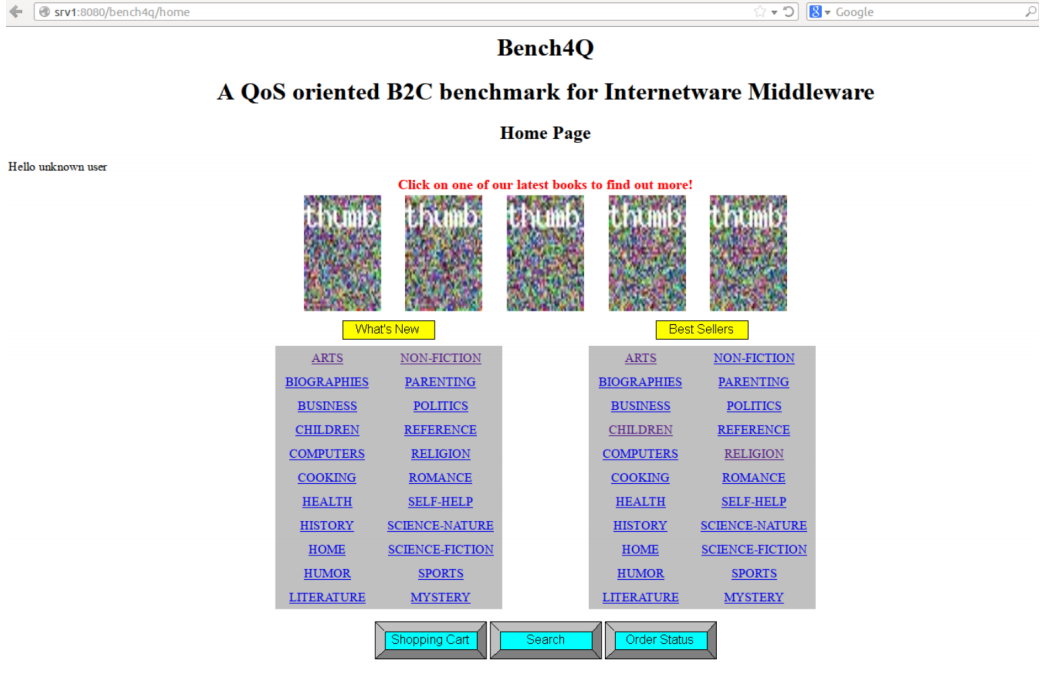
\includegraphics[scale=0.51]{sut.png}
		\caption{Bench4Q SUT}
		\label{fig:sut}
		\fdireta{Bench4Q}
	\end{figure}
	
\end{itemize}

De uma maneira mais especifica, percebe-se que os \textit{benchmarks} para aplicações computacionais típicas de computação em nuvem, como \textit{e-commerce}, por exemplo, não são atualmente orientados a suportar totalmente QoS, porque alguns recursos de QoS críticos não podem avaliados por eles \cite{Zhang2011}. Um exemplo desses recursos é a integralidade do serviço, que é geralmente expressa como uma sessão fornecido aos clientes. Nesse sentido o Bench4Q tenta abranger essa lacuna.


O TPC-W, estendido pelo Bench4Q, é (mesmo atualmente tido como obsoleto) um \textit{ benchmark} direcionado a \textit{sites} de \textit{e-commerce} transacionais em que os consumidores são vinculados a sessões, cada cliente possui sua própria e única sessão em determinado instervalo de tempo. Trata-se de um site de venda de livros implementado em Java e hospedado em um servidor de aplicação Tomcat \footnote{Tomcat: \url{http://tomcat.apache.org/}}. Clientes, intitulados pela ferramenta como \textit{browsers}, são emulados e se comportam como consumidores dos produtos oferecidos pela loja virtual. Basicamente, os clientes podem interagir de diferentes formas: acessar a página inicial do \textit{site} (home), navegar e procurar por produtos, realizar operações que envolvam o carrinho de compras e finalizar uma compra. A carga de trabalho gerada pelo TPC-W pode ser representada por um \sigla{CBMG}{\textit{Customer Behavior Model Graph}}, um grafo orientado, em que os nós representam uma operação a ser realizada (procurar, navegar, comprar etc.) e os pesos nas arestas significam a probabilidade de transição de uma operação para outra \cite{Zhang2011}. A Figura \ref{fig:CBMG} modela o fluxo de requisições a páginas e operações que um cliente pode realizar em uma sessão, basicamente um comportamento estocástico de acesso às páginas.

\begin{figure}[htb]
	\centering
	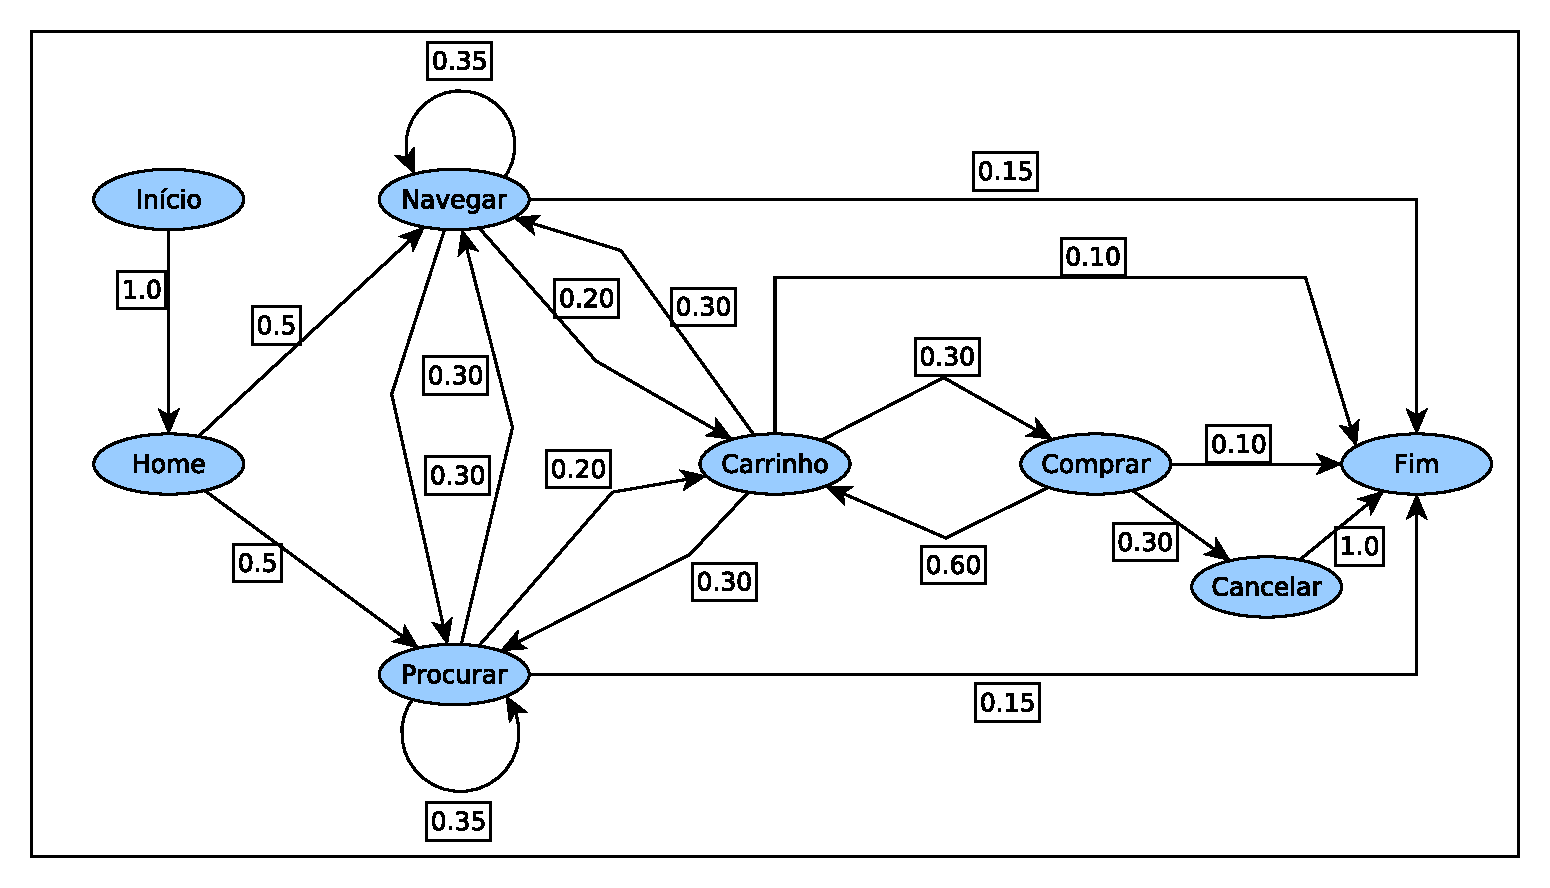
\includegraphics[scale=0.6]{CBMG.pdf}
	\caption{CBMG - perfil de navegação dos \textit{brwosers} do Bench4Q}
	\label{fig:CBMG}
	\fadaptada{Mark2007}
\end{figure}


A carga de trabalho gerada pelo TPC-W é formada por um CBMG com 14 tipos de interação \textit{web} e três perfis de pesos para suas arestas. O resultado é uma carga em que a maioria dos clientes apenas navega nas páginas (navegação: $95\%$ e compra: $5\%$); outra em que a maioria dos clientes realiza compras de forma moderada (navegação: $80\%$ e compra: $20\%$); e a terceira composta por muitos clientes que finalizam as compras (navegação: $50\%$ e compra: $50\%$). Vale ressaltar que existe um atraso entre as requisições de uma sessão. Ao iniciar uma sessão uma requisição é disparada e após receber a respectiva resposta, a próxima requisição acontece após um tempo também estocásticos e variante. Essa especificação tem o objetivo de emular melhor o comportamento humano ao acessar \textit{sites} de \textit{ e-commerce}.

Ao ser implantado em uma infraestrutura computacional que hospede todos seus componentes, os clientes emulados devem estar localizados fora de tal infraestrutura e conectados por uma rede. Os clientes começam as séries de requisições. O TPC-W implementa um modo de geração de carga conhecido como fechado (\textit{close mode}): um novo cliente chega somente após o antigo deixar o sistema \cite{Zhang2011}. As métricas disponíveis concernem basicamente sobre a quantidade de interações \textit{web}, medidas em quantidade por segundo (\sigla{WIPS}{\textit{ Web Interaction Per Second}}) e seu tempo de resposta (\sigla{WIRT}{\textit{Web Interaction Response Time}}).

A motivação para a extenção do TPC-W e criação do Bench4Q começa porque, muito embora, as referidas métricas aparentem descrever bem a quantidade de acessos ao sistema, a qualidade do serviço experimentada pelo usuário pode ser desproporcional a essas mesmas métricas. Em \cite{bench4qslides} é descrito um ensaio que contempla dois cenários diferentes: um normal e outro otimizado não realisticamente. A otimização foi feita pela configuração de parâmetros no servidor Tomcat, a saber: \texttt{sessionTimeout}, \texttt{connectionTimeout} e \texttt{acceptCount}. Um das características da aplicação é a presença de operações \textit{ IO-bound}, por consequência, observar o tempo médio de resposta dessas operações permite diminuir os valores de estouro de tempo, e, com isso, forçar uma taxa de utilização de CPU. Assim, pode-se ``otimizar'' o ambiente da aplicação. Os resultados foram de $WIPS = 131$ para o cenário normal e $WIPS=199$ para aquele otimizado não realisticamente, colaborando com a hipótese. Porém, ao observar a quantidade de sessões completadas com sucesso, conforme apresentado na figura \ref{fig:seeing}, percebe-se que o cenário normal permitiu uma quantidade de erros menor do que aquele otimizado não realisticamente. Por consequência, uma espectativa de lucro maior quando da implantação: maior quantidade de sessões realizadas sem error implicaria em maior probabilidade de compras efetivas.

\begin{figure}[htb]
	\centering
	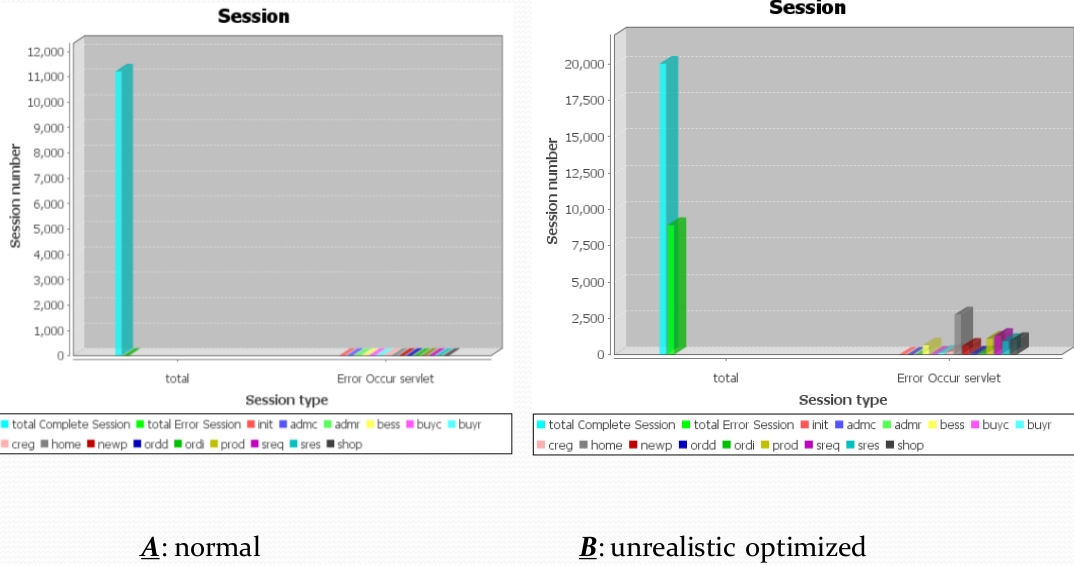
\includegraphics[scale=0.45]{seeing.png}
	\caption{Comparação da quantidade de requisições completadas com sucesso entre dois cenários: normal e otimizado não realisticamente.}
	\label{fig:seeing}
	\fdireta{Bench4Q}
\end{figure}


Tanto o TPC-W quando Bench4Q tem como objetivo produzir resultados que possibilitem o \textit{tuning} (sintonia do parâmetros) de servidores que compõem serviços de \textit{e-commerce} orientados a fornecer QoS aos seus clientes \cite{Menasce2002, Zhang2011}.  A ideia principal é que seja construída uma banca de testes (\textit{testbed}), haja a execução do \textit{ benchmark} e consecutiva geração dos traços de execução, seja feita a extração dos dados e, por fim, com base nos resultados, melhores valores para os parâmetros de configuração do sistema sejam aplicados. Especificamente sobre o Bench4Q, as principais funcionalidade implementadas nele tem como contexto a observância do estado das sesões.
%}

%Neste capítulo será apresentado o \textit{benchmark} Bench4q que foi desenvolvido pelo \textit{Technology Center of Software Engineering} da \textit{Chinese Academy of Sciences} no \textit{Institute of Software}.
O \textit{ e-commerce} é um modelo de negócio bastante comum e possível principalmente por sua implantação em ambiente \textit{ web}, orientado a negociação de bens e serviços. Igualmente como o que acontece na forma tradicional de negociação, disputas por clientes e/ou fatias de mecardo surgem naturalmente, como podem ser observadas em promoções, ofertas, lançamentos de novos produtos etc. Portanto, um \textit{ website} alinhado a esses requisitos que proporcionem um desempenho melhor, ou seja, que possibilidade uma experiência melhor a seus usuários, certamente já começa melhor. Nesse sentido, o desempenho da infraestrutura que hospedará o negócio e o ajuste fino dos parâmetros operacionais da solução de \textit{ e-commerce} podem ser encarados como requisitos não-funcionais. Assim, seria possível realizar avaliações de desempenho que fomentem o projeto de tais sistemas cujo resultado sejam sistemas mais eficientes, mesmo que sejam abstraídas algumas regras específicas do negócio a ser implementado. O Bench4Q é uma ferramenta que possibilita tais projetos.

A oscilação da carga de trabalho é uma característica fundamental. A simultaneidade dos acessos apresentam grandes efeitos sobre a escolha da política de ajuste de um servidor, o Bench4Q simular tal oscilação de carga atrás de seus agentes com os seguintes parâmetros:

\begin{itemize}
	\item \textit{Base Load:} Quantia fixa de \textit{threads} por agentes.
	\item \textit{Radom Load:} Quantidade de \textit{threads} que são geradas aleatoriamente.
	\item \textit{Rate:} O \textit{rate} (taxa de mudanças de carga), pode ser positivo, negativo ou nulo. Positivo significa que a carga de base está aumentando a cada segundo, se negativa significa que a carga de base está diminuindo a cada segundo e enquanto a taxa é zero, a carga é fixa.
	\item \textit{Trigger Time:} O tempo para o agente de carga para começar a gerar sua carga.
	\item \textit{Duration:} O tempo de execução do agente de carga.
\end{itemize}

As composições as cargas simuladas por diversos agentes, podem gerar as seguintes flutuações de carga típicas de empresas B2C podem ser simulados.

\begin{figure}[htb]
	\centering
	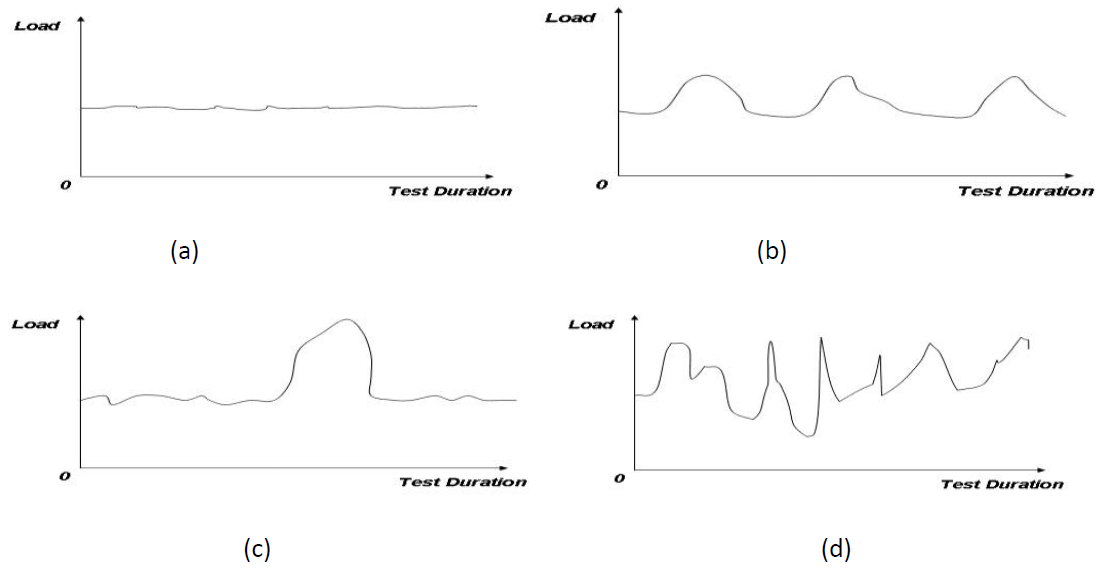
\includegraphics[scale=0.5]{load_fluctuation.png}
	\caption{Carga de trabalho gerada pelo Bench4Q}
	\label{fig:carga-gerada}
	\fdireta{Bench4Q}
\end{figure}


Existe dois modos de simulação de carga, o fechado e o aberto, conforme apresentado na figura \ref{fig:type-session}. No modo fechado, ilustrado na figura \ref{fig:type-session} (a), um novo cliente só acessará depois de cliente antigo deixar o sistema. Já o modo aberto, ilustrado na figura \ref{fig:type-session} (b), novos clientes vão acessar o sistemas sem se importa  com a saída dos antigos clientes. O TPC- W simula carga no modo fechado, o que faz uma suposição inexistente do mundo real \cite{Bench4Q}. 

\begin{figure}[htb]
	\centering
	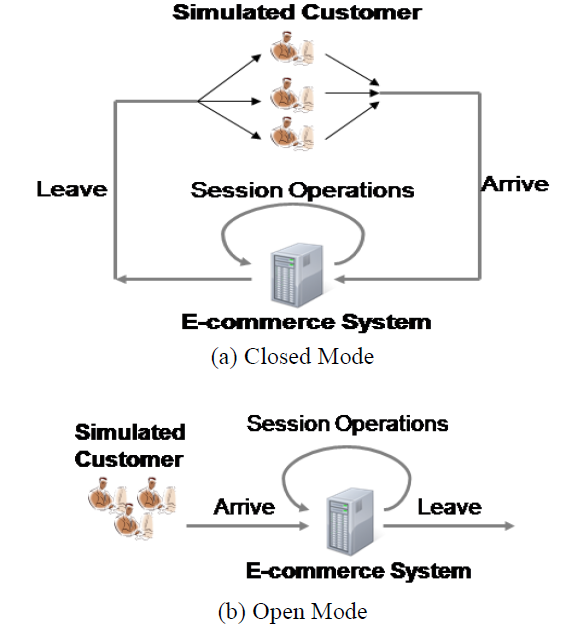
\includegraphics[scale=0.6]{type_session.png}
	\caption{Tipo de sessões Bench4Q}
	\label{fig:type-session}
	\fdireta{Bench4Q}	
\end{figure}


Em sistemas baseados em sessões reais, como a proposta deste projeto, os clientes vêm com base em um modo aberto. Em sua utilização neste projeto, a sessão aberta é a que mais se adéqua a finalidade do objetivo proposto pelo trabalho.


%definição para fisicos - Dynamical systems in cosmology
%O que é um sistema dinâmico? Pode ser qualquer coisa que vão desde algo tão simples como um único pêndulo para algo tão complexo como o cérebro humano e todo o próprio universo. Em geral, um sistema dinâmico pode ser considerado como qualquer sistema que consiste em resumo
%1. um espaço (espaço de estados ou espaço de fase), e
%2. uma regra matemática que descreve a evolução de qualquer ponto nesse espaço.
%O segundo ponto é crucial. Encontrar uma regra matemática que, por exemplo, descreve a evolução da informação em qualquer neurônio no cérebro humano é provavelmente impossível. Então, precisamos de uma regra matemática como uma entrada e encontrar um pode ser muito difícil.
%O estado do sistema, estamos interessados ​​em é descrito por um conjunto de quantidades que são considerados importantes sobre o sistema, eo espaço de estado é o conjunto de todos os valores possíveis destas quantidades. No caso do pêndulo, a posição da massa e a sua quantidade de movimento são quantidades naturais para especificar o estado do sistema. Para sistemas mais complicados, como o universo como um todo, a escolha de boas quantidades não é de todo óbvio e ele acaba por ser útil para escolher variáveis ​​convenientes. É possível analisar o mesmo sistema dinâmico com diferentes conjuntos de variáveis, cada um dos quais pode ser mais apropriado a uma questão particular.
%Existem dois tipos principais de sistemas dinâmicos: A primeira são sistemas dinâmicos contínuos cuja evolução é definida por um conjunto de equações diferenciais ordinárias (EDOs) e os outros são chamados de sistemas dinâmicos em tempo-discreto que são definidos por um mapa ou equações de diferença. No contexto da cosmologia estamos estudando as equações de campo de Einstein que para um resultado homogêneo e isotrópico espaço em um sistema de equações diferenciais ordinárias. Assim, estamos interessados ​​apenas em sistemas dinâmicos contínuos e não discutirá sistemas dinâmicos em tempo-discreto no restante


% Nobile
%Em geral, é possível representar sistemas físicos (e. g. eletrônicos, químicos e biológicos) por equações diferenciais obtidas a partir leis básicas da Física. Esses sistemas de equações diferenciais descrevem uma determinada dinâmica do sistema no domínio do tempo e, com o desenvolvimento dessas equações, é possível identificar propriedades fundamentais para o projeto de controle.
%Nas engenharias sistemas mecânicos são bastante semânticos e amplamente utilizados como exemplo na modelagem de sistemas. A figura 3.5 ilustra um sistema mecânico massa-mola simples onde um objeto de massa m está preso a uma mola cuja constante de elasticidade é igual a k fixa em uma superfície plana. Para simplificar a modelagem, considerações podem ser feitas, como supor que o sistema está livre da influência de outras forças.


%\cite{mytkowicz2009} afirma que  computadores modernos são sistemas dinâmicos não-lineares

%_____________Computer systems are dynamical systems
%Os computadores modernos são sistemas dinâmicos não-lineares complexas. Registos microprocessador, o conteúdo da memória, e até mesmo a temperatura de diferentes regiões do chip são variáveis ​​de estado desses sistemas. A lógica programado em um computador, combinados com o software de execução em que o hardware, define a dinâmica do sistema. Sob a influência dessas dinâmicas, o estado do computador se move em uma trajetória através do seu espaço de alta dimensão estado como o progresso ciclos do relógio eo programa é executado. Chamamos isso a dinâmica de um sistema de computador de desempenho para distingui-lo a partir da dinâmica do programa: a sequência de passos que o código a seguir. Embora a dinâmica do programa são geralmente simples e fácil de entender, a dinâmica de um programa rodando em um computador moderno de desempenho pode ser complexo e até mesmo caótico. As implicações disso não são apenas interessante, mas realmente muito importante, tanto do ponto de vista dinâmica e para os efeitos de simulação computacional e design.
%Este pensamento está em contraste gritante com as abordagens tradicionais na literatura sistemas de computadores, onde os computadores são modeladas como processos estocásticos altos-dimensional, 1,2 detalhes temporais estão aglomeradas em indicadores agregados, 3,4 e os problemas de observação e de perturbação que são inerentes em qualquer experiência do mundo real são evitados através da utilização de simuladores, em vez de hardware.5,6 real dos 364 trabalhos sobre a compreensão do desempenho de inovações microprocessador que apareceu entre 2004 e 2007, em três conferências microarquitetura importantes? ASPLOS, ISCA, e micro ?, por exemplo, apenas nove analisaram o comportamento variável no tempo de hardware real. Enquanto arquitetos de computador fazem perceber os efeitos de não-linearidade, falta-lhes um quadro verdadeiramente princípios para lidar com seus efeitos. Como uma solução parcial, o campo tem utilizado abordagens baseadas no conhecimento? Por exemplo, refs. 10/07? e técnicas fundamentadas em pesquisa e operações de investigação? por exemplo, refs. 11-13 ?. Mesmo assim, o resultado de um novo recurso de design rotineiramente surpreende sua creators.14
%A combinação particularmente pernicioso de não-linearidade e medição perturbação só recentemente foi reconhecido como uma questão importante por computador architects.15,16 computadores modernos têm milhões de transistores que interagem de formas complexas e não-lineares, e quase qualquer medição de seu estado pode perturbar o seu comportamento . Como resultado, a dinâmica de sistemas de computadores de desempenho pode olhar random-dando assim origem e credibilidade à idéia de que a evolução do desempenho de um computador acontece a partir de um processo estocástico.
%Como os leitores desta revista estão bem conscientes, no entanto, olhando aleatória e ser aleatório pode ser duas coisas diferentes. A dinâmica de um computador é ditada pelas leis físicas determinísticos de suas partes: fios, semicondutores, e assim por diante. Nem este hardware nem o código que é executado em que é estocástico, e assim parece lógico ter uma abordagem dos sistemas dinâmicos para a análise do seu comportamento acoplado.
%Seguindo este raciocínio, nós tratamos a tarefa de compreender o comportamento de um computador como equivalente a análise da dinâmica de espaço de estado do sistema. Esta abordagem, foi pioneira na Ref. 17, não é apenas uma maneira útil de descrever e compreender estes sistemas; ele também permite-nos comparar dois sistemas desse tipo, o que é essencial para a tarefa de modelagem e validação de seu comportamento. Indo além do trabalho em Ref. 17- que calculou invariantes dinâmicos de complexos programas de computador que funcionam em computadores simulados-formulamos um modelo geral para a dinâmica de computador, sob a forma de um mapa iterado, e validá-lo usando dois tipos diferentes de computadores Intel. Estudar a dinâmica de hardware real é crítica porque simuladores raramente correspondem sistemas reais, mas levanta alguns desafios significativos aqui. Como é o caso em muitos experimentos de laboratório, é impossível medir todas as variáveis ​​de estado de um computador que executa e difícil de evitar perturbar aqueles que podem ser medidos. O delineamento experimental também é crítica; sistemas de computador são feitas de vários módulos de hardware e software, alguns dos quais não estão sob controle explícita do usuário, mantendo assim todas as condições constante requer cuidados real. Nós usamos uma infra-estrutura de medição personalizado para resolver estes problemas e coletar dados de série temporal que reflete o desempenho de um computador em funcionamento. Nós empregamos atraso de coordenar a incorporação desses dados para reconstruir a dinâmica de vários programas de computador em execução em duas máquinas físicas diferentes. Analisamos as diferentes influências sobre a dinâmica, demonstrando que tanto hardware e software jogo complicado, funções não-lineares no comportamento dos sistemas, e nós fornecemos a primeira evidência experimental de dinâmica caótica de baixa dimensionalidade em hardware de computador real. Mostramos também que a dinâmica de um computador é submetido a uma série contínua de bifurcações como a execução se move através de diferentes partes do código.
%É importante notar que nem toda essa complexidade dinâmica e manifesto riqueza a menos que alguém estuda um computador real, não apenas um simulador que imita seu comportamento-a abordagem comum em trabalhos anteriores sobre este tema, tanto na arquitetura de computadores e sistemas dinâmicos literaturas. Simuladores são muito atraentes para estudar porque se pode facilmente medir todas as suas variáveis ​​de estado e porque o seu comportamento é repetitivo. Eles são versões de computadores reais altamente simplificada, porém, e sua partida para esses sistemas é cada vez mais posta em causa pela comunidade arquitetura de computador? Por exemplo, Ref. 5 ?. O comportamento de hardware real não é completamente reprodutíveis, 16 e melhorias de design que são trabalhados para fora usando simuladores muitas vezes provar ter efeitos inesperados quando são implementadas em silício e metal.14 Nada disto é surpreendente; captar bem a dinâmica de um sistema de vários milhões de transistor com algumas dezenas de milhares de linhas de código? por exemplo, como nas refs. 18 e 19? é difícil, se não impossível. Por todas estas razões, é fundamental para estudar os computadores reais, não os simulados.
%O trabalho descrito neste artigo é não só uma interessante aplicação de técnicas de dinâmica não linear para uma nova área de aplicação. Ele representa um completamente novo ângulo de ataque em alguns dos problemas mais prementes que da área de aplicação.
%Atualmente, por exemplo, os simuladores que são empregados por arquitetos de computadores são validados apenas usando métricas end-to-end, como o tempo de execução de um programa, 4 e eles raramente são comparados de forma alguma dinâmica significativa para os sistemas reais que eles são supostos para imitar. Os resultados aqui apresentados deixar claro que indicadores agregados são insuficientes e os detalhes da dinâmica importa: Dois sistemas de computador devem ser tratados como semelhante, se e somente se os seus invariantes dinâmicos combinam. Isto põe em causa a noção de validação simulador e explica algumas das resultados que têm assustado os arquitetos de computadores ao longo dos anos, quando ocorre uma melhora de design que foi trabalhado em um simulador saiu mal em hardware.14 reais
%Nossos resultados nos levam a uma vista de um computador como um sistema dinâmico que opera sob a influência de uma série de bifurcações induzidas pelo código que está sendo executado. Isto sugere que a análise bifurcação pode ser útil na identificação de diferentes regimes de comportamentais em um programa de computador e que invariantes dinâmicos podem ser úteis para a análise do comportamento em cada regime. Este ponto de vista também explica alguns dos resultados inconclusivos em Ref. 17, como no mundo real programas de computador são uma mistura complexa de múltiplos atractores e comportamento transiente, e o cálculo de um dinâmico "invariante" de uma tal trajectória pode ser problemático. No quadro mais amplo, nossos resultados sugerem que não se pode compreender o comportamento de um computador por entender como a função de hardware e subsistemas de software e, depois, compor as suas dinâmicas. Em vez disso, deve-se tratar o sistema como uma rede de complexo, não linear, interagindo peças de CPU, cache, memória de acesso aleatório? RAM ?, disco, placas de vídeo, sistema operacional, os programas do usuário, etc., e analisar a dinâmica resultante como uma todo.


%Este trabalho propõe uma metodologia de extensão de analise transiente para \textit{benchmarks}, levando isso em consideração o grupo 3 (Requisitos de Carga de Trabalho - contém os requisitos quanto à definição de carga de trabalho e suas interações.) é o que melhor se adequá para as necessidade de uma analise transiente. Sendo assim todos os itens presente neste grupo 3 são pré-requisitos para metodologia de extensão. 
%Diante nas necessidades é importante incluir mais um item tão importante quando os outros, mas com intenção diferente em comparação aos outros. Será necessário alterar o código fonte do gerador de carga, logo o \textit{benchmark} deve ser \textit{Open-source} ou a equipe que aplicará as modificações e consequentemente a metodologia deve ter permissão para modificar ou ter acesso ao código fonte.


%\begin{itemize}
%	\item \textit{Open-source} ou ter acesso ao código fonte para as modificações
%	\item possuir um gerador de carga
%	\item Ter na composição ou poder incluir um sistema para avaliação	
%	\item Ter ou possibilitar a inclusão de métrica(s) de caráter transiente
%\end{itemize}

\begin{comment}
Afim de exemplificar, a tabela \ref{table:benchmarks} lista um conjunto de \textit{benchmarks} e verificamos a existências dos pré-requisitos definidos para a metodologia, vale salientar que todos os \textit{benchmarks} não apresentam qualquer analise em regime transiente que o alvo deste trabalho.

\begin{center}
	\label{table:benchmarks}
	%\caption{Lista de \textit{benchmark} com pré-requisitos}
	\begin{longtable}{| m{2cm} | m{1.5cm} | m{1.7cm} | m{2cm} | m{1.5cm} | p{5.5cm} |}
		\hline
		\textbf{\textit{Benchmarks}} & \textbf{Open-source} & \textbf{Gerador de carga} & \textbf{Sistema de avaliação} & \textbf{Métricas} & \textbf{Resumo}
		\\ 
		\hline
		\textbf{Bench4Q} & \thereIs & \thereIs & \thereIs & \thereIs & Bench4Q, é um \textit{e-commerce} orientada QoS, tem recursos para deduzir uma representação controlável e flexível de cargas de trabalho baseadas em sessão complexas, e para simular o comportamento do cliente autêntico. %Além do mais, o Bench4Q pode ser utilizado para avaliar o desempenho e escalabilidade do sistema. 
		\\ 
		\hline
		\textbf{DynBench} & \thereIs & \thereIs & \thereNotIs & \thereIs & DynBench é útil para avaliação QoS e/ou Gestão de Recursos em sistemas de tempo real distribuídos. Como tal, DynBench inclui um conjunto de métricas de desempenho para a avaliação de QoS e tecnologias Gestão de Recursos.\cite{Shirazi1999}
		\\ 
		\hline
		\textbf{EEMBC} & \thereIs & \thereIs & \thereNotIs & \thereIs & EEMBC atende às necessidades dos projetistas de sistemas embarcados, fornecendo um conjunto diversificado de benchmarks de processadores organizados em categorias que abrangem inúmeras aplicações do mundo real. 
		\\ 	
		\hline
		\textbf{LinkBench} & \thereIs & \thereIs & \thereIs & \thereIs & LinkBench é uma referência de banco de dados desenvolvido para avaliar o desempenho do banco de dados para cargas de trabalho semelhantes às da produção implantação MySQL do Facebook 
		\\ 	
		\hline
		\textbf{OLTP} & \thereIs & \thereIs & \thereNotIs & \thereIs & OLTP, é um extensível que é adaptado para o processamento on-line de transações (OLTP) e cargas de trabalho orientadas para a web.
		\\ 	
		\hline
		\textbf{RUBiS} & \thereIs & \thereIs & \thereIs & \thereIs & Rubis é um protótipo de site de leilão modelado após eBay.com que é usado para avaliar os padrões de design de aplicativos e escalabilidade de desempenho de servidores de aplicação.
		\\ 
		\hline
		\textbf{SWIM} & \thereIs & \thereIs & \thereNotIs & \thereIs & SWIM permite uma medição rigorosa de sistemas desenpenho de MapReduce. SWIM contém conjunto de cargas de trabalho, com dados complexos e chegada e padrões de computação. 
		\\ 
		\hline
		\textbf{TPC-W} & \thereIs & \thereIs & \thereIs & \thereIs & TPC-W especifica uma carga de trabalho de comércio eletrônico que simula as atividades de um site \textit{e-commerce}.
		Emulada usuários que podem navegar e encomendar produtos do site. \cite{Menasce2002}
		\\ 		
		\hline
		\textbf{YCSB} & \thereIs & \thereIs & \thereIs & \thereIs & com o objectivo de facilitar as comparações de desempenho da nova geração de sistemas de nuvem de dados. o YCSB é uma ferramenta que ela é extensível e suporta fácil definição de novas cargas de trabalho. \cite{Cooper2010}
		\\ 
		\hline
	\end{longtable}
\end{center}
\end{comment}








\chapter{Metodologia}
\label{chapter:metodologia}
\begin{frame}{Parâmetros para moduladar a carga}
	\begin{itemize}
		\item \textbf{Tempo de planejamento de carga:} Um período de tempo em que a carga de trabalho é modulada, caracterizando a mudança do comportamento das requisições de maneira programada;
		
		\item \textbf{Tipo de modulação:} a modulação será apresentada conforme as funções ou sinais propostos por \cite{Hellerstein2004};
		
		\item \textbf{Tempo de interrupções:} Período de interrupções/pausa após o \textit{Tempo de planejamento de carga};
		
		\item \textbf{Quantidade de clientes na modulação:} reservar uma quantidade de clientes EBs, que estão com dedicação exclusiva para a modulação da carga.
	\end{itemize}	
\end{frame}

\begin{frame}{Possibilidade de cargas moduláveis pela extensão}
	\begin{columns}
		\column{0.5\textwidth}
		\begin{minipage}[c][0.4\textheight][c]{\linewidth}
			\centering
			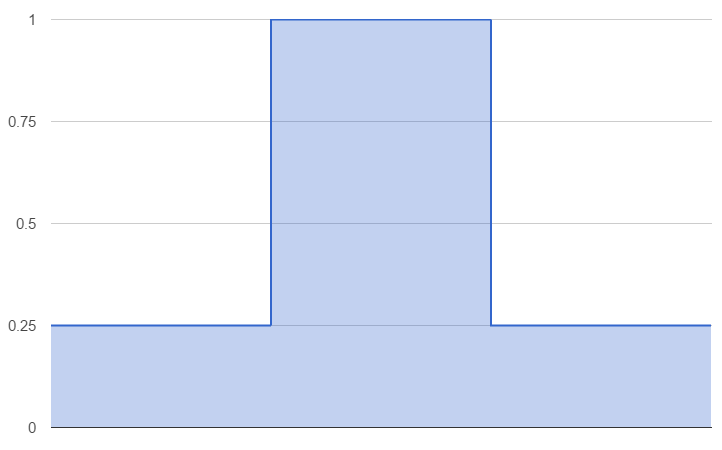
\includegraphics[width=0.8\linewidth]{../monograph/images/carga-sintetica1.png}
			\label{fig:degrau-positivo}
		\end{minipage}
		\begin{minipage}[c][0.4\textheight][c]{\linewidth}
			\centering
			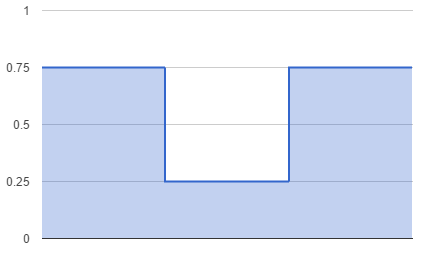
\includegraphics[width=0.8\linewidth]{../monograph/images/carga-sintetica2.png}
			\label{fig:degrau-negativo}
		\end{minipage}
		\column{0.5\textwidth}
		\begin{minipage}[c][0.4\textheight][c]{\linewidth}
			\begin{enumerate}
				\item Degrau positivo,
				\item Degrau negativo,
				\item Onda quadrada;
			\end{enumerate}
		\end{minipage}
		\begin{minipage}[c][0.4\textheight][c]{\linewidth}
			\centering
			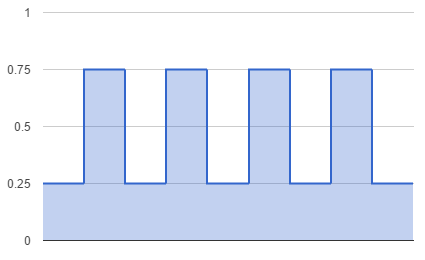
\includegraphics[width=0.8\linewidth]{../monograph/images/carga-sintetica3.png}
			\label{fig:onda-gradrada}
		\end{minipage}
	\end{columns}
\end{frame}

\begin{frame}{Arquitetura do experimento}
	\begin{columns}
		\column{0.4\textwidth}
		\begin{minipage}[c][0.4\textheight][c]{\linewidth}
			\centering
			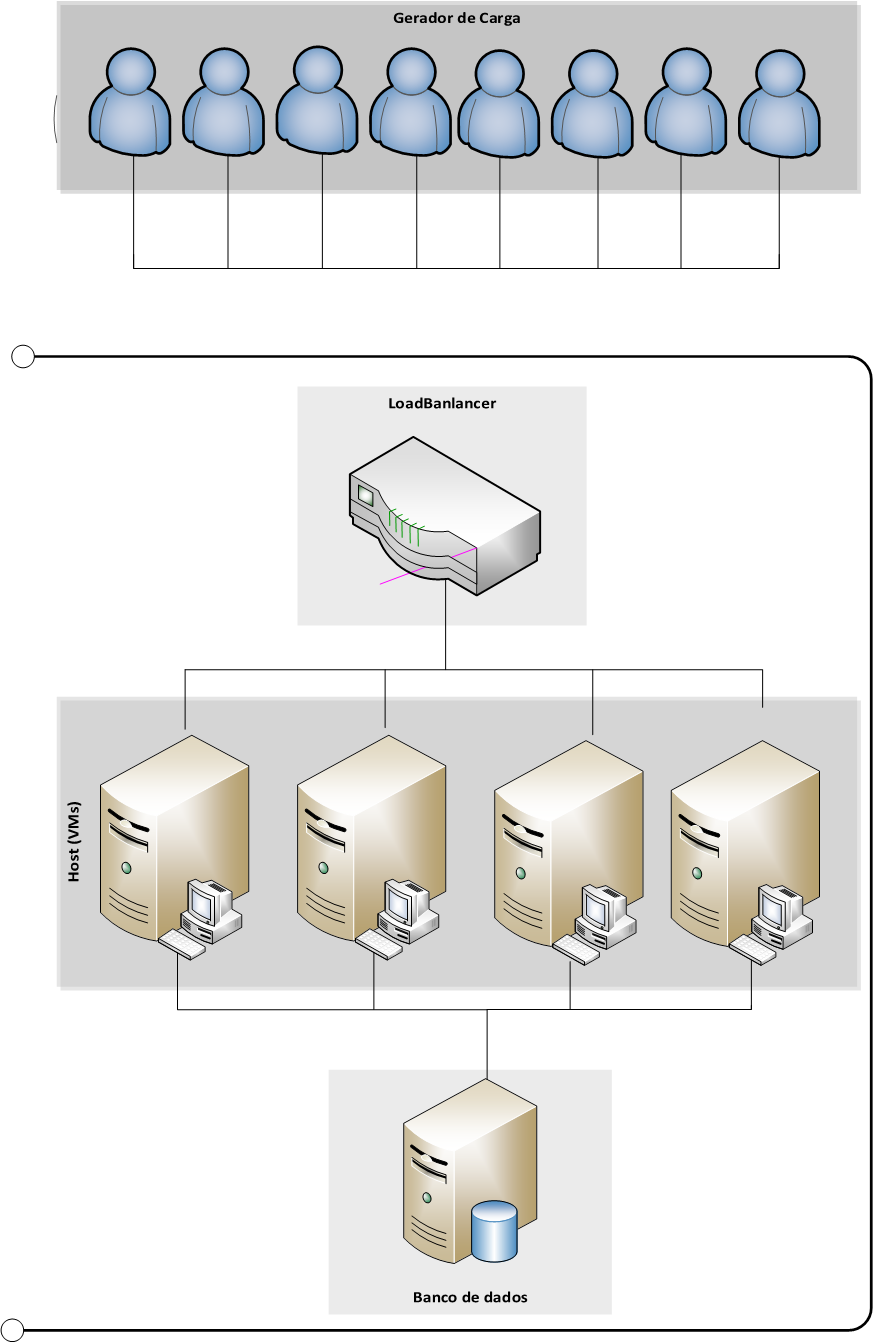
\includegraphics[scale=0.17]{../monograph/images/arquitetura-experimento.png}
			\label{fig:arquitetura-experimento}		
		\end{minipage}
		\column{0.6\textwidth}
		\begin{minipage}[c][0.4\textheight][c]{\linewidth}
			\begin{itemize}
				\item Gerador de Carga (\textit{Workload})
				\item Balanceador de carga (\textit{Load Balancer})
				\item Servidor Físico (\textit{Hypervisor})
				\item Servidor de dados (\textit{Data base})
			\end{itemize}
		\end{minipage}		
	\end{columns}
	
\end{frame}

\begin{frame}{Comportamento de métrica transiente}

\end{frame}

\begin{frame}{Comportamento de métrica transiente}
	\begin{columns}
		\column{0.45\textwidth}
		\begin{minipage}[c][0.45\textheight][c]{\linewidth}
			\centering
			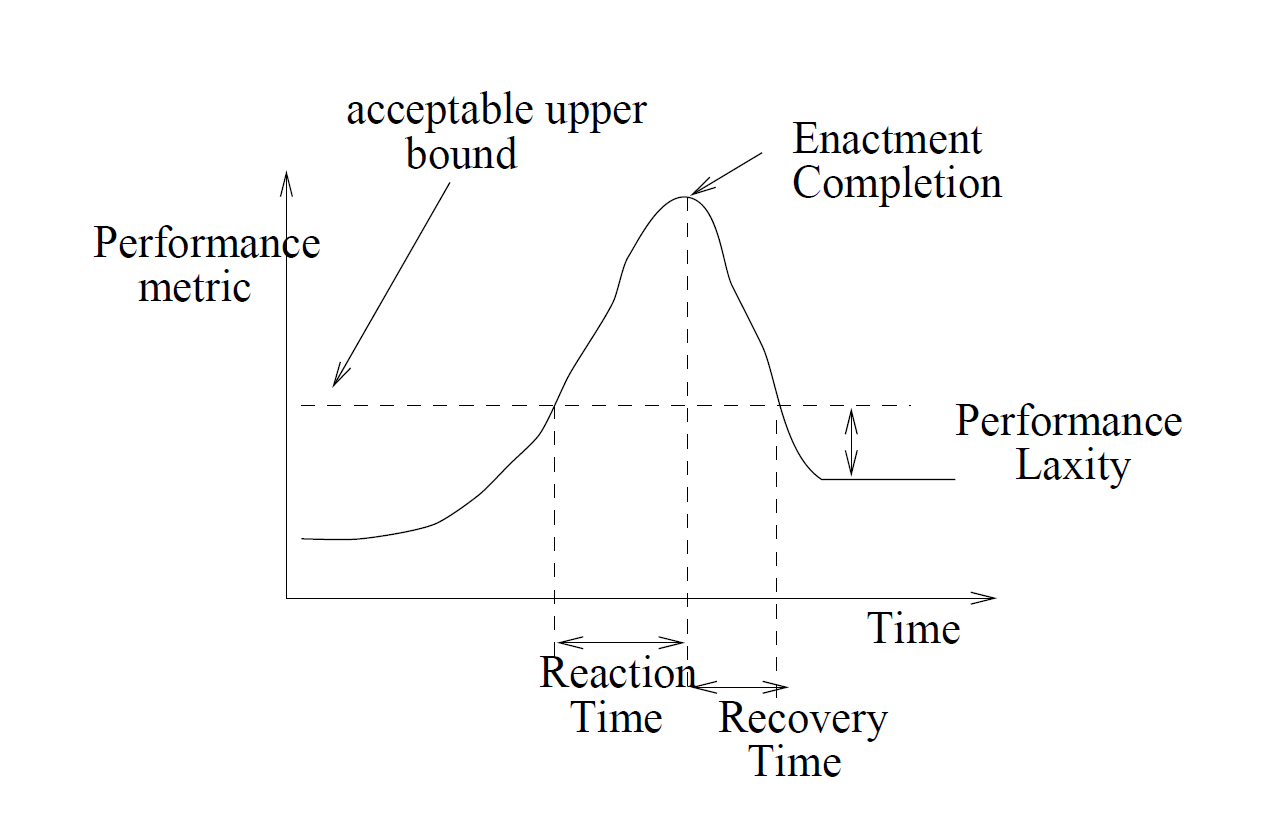
\includegraphics[width=1.27\linewidth]{../monograph/images/transient-metric.png}
			\label{fig:transient-metric}	
		\end{minipage}
		\column{0.55\textwidth}
		\begin{minipage}[c][0.55\textheight][c]{\linewidth}
			\begin{itemize}
				\item \textbf{\textit{Reaction Time} (Tempo de reação)} - o período entre a ocorrência da variação crítica e a conclusão da promulgação realocação de correção;
				
				\item \textbf{\textit{Recovery Time} (Tempo de Recuperação)} - o intervalo entre a conclusão, promulgação e da restauração de um nível de desempenho aceitável;
				
				\item \textbf{\textit{Performance Laxity} (Frouxidão performance)} - a diferença entre o \textit{required vs performance}, e o desempenho em estado estacionário, após a redistribuição;
			\end{itemize}
		\end{minipage}		
	\end{columns}
\end{frame}

\begin{frame}{Métrica transiente}
	\begin{itemize}
		\item \textbf{Conexões por segundo (\textit{Load Balancer}):} Conforme sugerido por \cite{Binnig2009}, medir a escalabilidade através do aumento dos interações web emitidos por segundo ao longo do tempo e de forma contínua contando a interação web que são respondidas em um intervalo de tempo de resposta,
		
		\item \textbf{Tempo de resposta (\textit{browsers}):} \cite{helder2014}, em um sistema dinâmico, cuja transformação entrada-saída não ocorre em tempo zero, mas é sujeita a uma inércia advinda dos processos físicos associados, possuí uma inércia intrínseca que atrasa o efeito que uma entrada terá na saída. Esses efeitos refletem no consequentemente nos comportamentos diversos que incluem retardo no tempo de resposta e possíveis oscilações; 	
	
	\end{itemize}
\end{frame}

\begin{frame}{Métrica transiente}
	\begin{itemize}
		\item \textbf{Taxa de utilização da CPU (VMs):} \cite{Nobile2013} afirma que diversas métricas podem ser analisadas para verificar o desempenho das máquinas virtuais, e cita alguns exemplos, como o tempo de inicialização, a taxa de utilização de CPU, o tempo médio de resposta e o \textit{throughput}, e usualmente, número de máquinas virtuais que hospedam serviços de interesse ao cliente e que respondem a uma carga de trabalho imposta por usuários através de requisições;
		
		\item \textbf{Taxa de utilização da CPU:} O trabalho apresentado por \cite{wang2009}, que lida com uma carga de trabalho variante no tempo e intensiva, demonstra que a CPU e I/O podem ser utilizadas para prever as necessidades dos recursos de um banco de dados e para orientar a alocação de recursos \textit{on-demand} de acordo com a exigência de carga de trabalho. Entretanto iremos somente considerar em nossos experimento a taxa de utilização do banco de dados.
	\end{itemize}
\end{frame}

\begin{frame}
	PEGAR IMAGEM DO EDWIN QUE EXPLICA A RESERVAR DOS EBs
\end{frame}



\chapter{Desenvolvimento}
\label{chapter:desenvolvimento}
Nesta seção é apresentado em detalhes a implementação aplicada no \textit{benchmark} Bench4Q. A Figura \ref{fig:diagrama-classes} mostra o diagrama de classes envolvido na extensão do Bench4Q. As classes sinalizadas na cor azul, representam as já existentes mas que passaram por adaptações e modificações, já as classes na cor verde, referem-se as novas classes criadas para possibilitar a modulação da carga do \textit{benchmark}.

Apesar de permitir a geração de carga para o sistema, o Bench4Q possui algumas limitações na sua versão original que dificultam a experimentação e analise de cenários de interesse ao trabalho de \citeonline{Edwin2015} e \citeonline{Lourenco2015} de quem pretende desenvolver técnicas de gerenciamento de recursos.
As classes disponíveis no \textit{benchmark} original não permitem a modulação de carga de trabalho, essa limitação implica, por exemplo, na dificuldade de projetar um controlador para o gerenciamento de recursos, pois para esta atividade é necessário uma análise de resultados transientes mediante a modulação da carga de trabalho. A simulação de uma carga de trabalho em que há a alteração introduzida ao longo da simulação é o foco deste trabalho.

\begin{figure}[!htb]
	\centering
	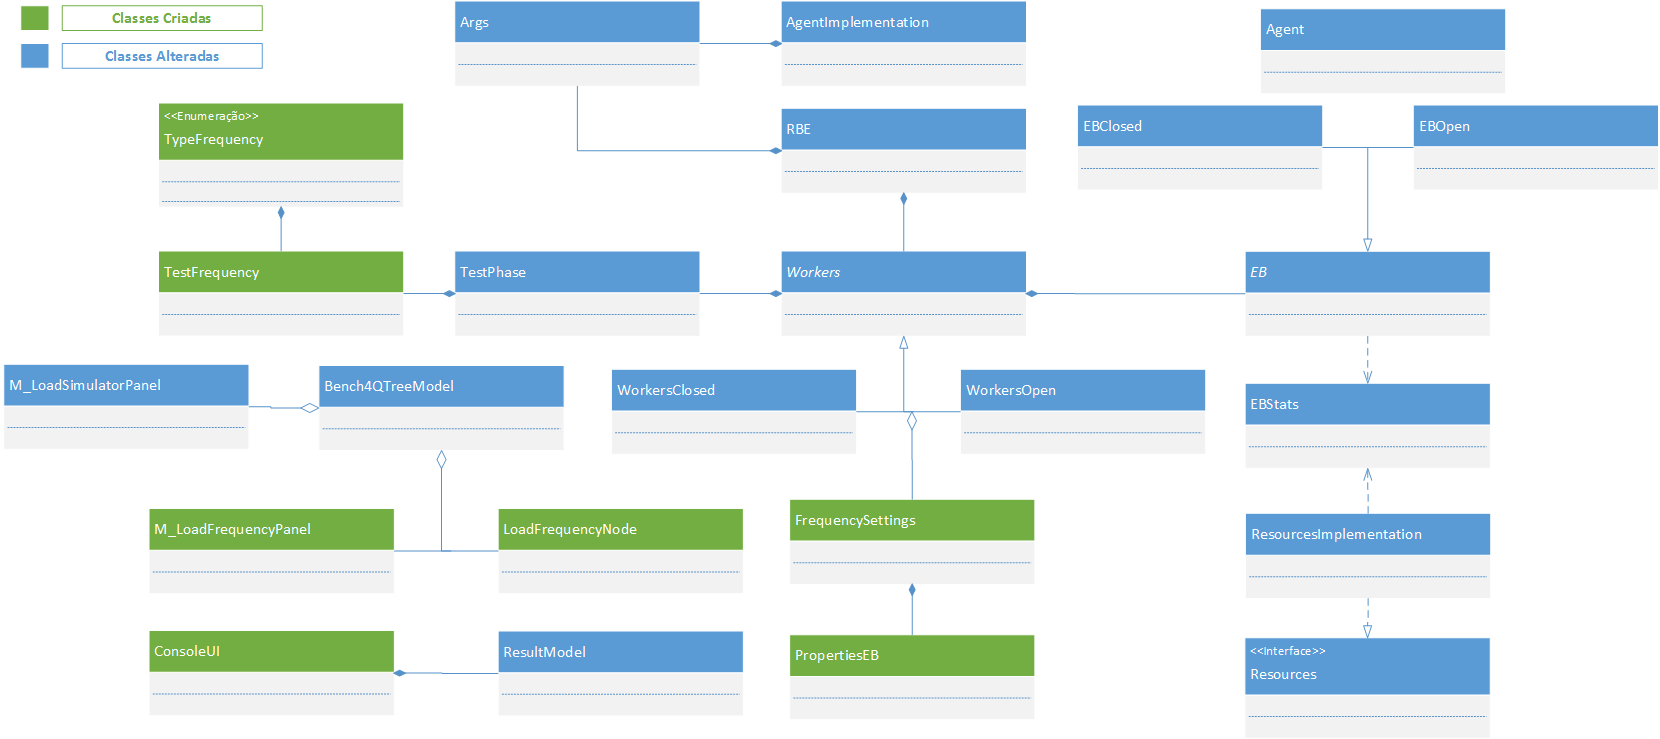
\includegraphics[angle=90, scale=0.6]{diagrama-classes-beanch4Q.png}	
	\caption{Diagrama de classes da extensão do Bench4Q.}
	\label{fig:diagrama-classes}
	\fautor
\end{figure}

Para distribuir a submissão da carga de trabalho ao longo da simulação, uma estratégia utilizada é a modulação da mesma através de parâmetros que configuram o comportamento da carga. O Bench4Q também não suporta nativamente a alocação e a deslocação dos recursos em tempo de simulação, uma conjunto de implementações foram necessárias para estender o \textit{benchmark}, essas aplicações não lidam com a modulação da carga de trabalho, mas manipulação a distribuição da carga de trabalho em um conjunto de servidores, da mesma maneira que um ambiente de nuvem, assim como o gerenciamento dos recursos da proposta de arquitetura. Contudo, os detalhes dessa implementação não serão apresentados e discutidos neste trabalho, uma vez este contexto foge do foco e da proposta do trabalho que tem por objetivo a modulação da carga.



%1º  - falar como foi implementados as modificações conforme a metodologia

A princípio foi identificado o modulo de geração de carga do Bench4Q e este passou por alterações para gerar a carga de trabalho esperada. Conforme o diagrama de classes na Figura \ref{fig:diagrama-classes}, é possível ter uma ideia do trabalho de extensão realizado no \textit{benchmark}, vale aqui salientar que o Bench4Q é uma ferramenta completa e extensa, e diagramar todas as classes do mesmo ficaria difícil e aumentaria consideravelmente a complexidade de entendimento, sendo assim, aqui apresentamos somente as classes já existem no Bench4Q e que passaram por modificações para atender aos requisitos da proposta, juntamente com as novas classes que foram necessárias para almejar o mesmo objetivo.

O Bench4Q fornece uma estrutura e componentes compartilhados para a comunicação entre os dois módulos da carga de trabalho, \textbf{Console} e \textbf{Agente}. Apesar de trabalharem em conjunto e para um mesmo fim, cada modulo (Console e Agente) é executado em máquinas distintas.  A extensão é construída inicialmente sob a classe \textsf{MLoadSimulatorPanel}, que orquestra toda a interatividade gráfica do Bench4Q. O novo painel de configuração, que modula a carga, \textsf{MLoadFrequencyPanel} estende da classe original \textsf{Bench4QTreeModel}, adicionando os parâmetros para a modulação: tipo da carga, o instante em que a carga se inicia, o tempo de atuação da carga e a quantidade de EBs que atuaram nessa carga. O parâmetro \textit{"tipos de carga"}, utiliza da classe enum \textsf{TypeFrequency} que define as constantes dos tipos de modulações programadas para esta extensão.  Todos os parâmetros inseridos na \textsf{MLoadSimulatorPanel} são armazenados na classe \textsf{TestFrequency} que se tornou uma propriedade da classe nativa \textsf{TestPhase}, que posteriormente são repassadas para a classe \textsf{PropertiesEB} através da \textsf{FrequencySettings}. Já nas classes \textsf{Agent}, \textsf{EB}, \textsf{EBClose}, \textsf{EBOpen}, \textsf{Workers}, \textsf{WorkersClosed} e \textsf{WorkersOpen} foram modificadas para receber os novos parâmetros da \textsf{PropertiesEB} e compreendê-los correspondentemente a modulação configurada na interface gráfica e gerando a carga programada durante a execução.

O código-fonte \ref{code:modelworkload}, é um pseudo-código que ilustra o esqueleto de maneira simplificada do \textit{core} da geração da carga referente a construção da modulação da carga já com as modificações da extensão.

\begin{codigo}[caption={Algoritmo de geração de carga modificado para modulaçao}, label={code:modelworkload}, breaklines=false]
ParametrosExperimento parametros;
	
ebCorrente.EmExecucao = true;
while (parametros.ExperimentoEmExecucao) {
		
	tempoCorrente = System.pegaTempoCorrente();
	
	if (tempoCorrente > parametros.TempoExperimento){
		ebCorrente.EmExecucao = false;
	}
	
	if (tempoCorrente > ebCorrente.TempoDuracao && ebCorrente.EbMarcado) {
		if(parametros.TempoPausa > 0){
			
			long novoInicio = ebCorrente.TempoFinal + parametros.TempoPausa ;
			long periodo = ebCorrente.TempoFinal - ebCorrente.TempoInicial;
			
			ebCorrente.TempoInicial = novoInicio;
			ebCorrente.TempoFinal = periodo + novoInicio;
		} else if (tempoCorrente > ebCorrente.TempoInicial) {
			ebCorrente.EmExecucao = false;
		}
	}

	if (tempoCorrente >= ebCorrente.TempoInicio) {
		if (!ebCorrente.EmExecucao) {
			return;
		}
		if (ebCorrente.TemProximaPagina) {
			// fluxo de acesso a pagina do SUT (recurso nativo do Bench4Q)
		} else {
			ebCorrente.EmExecucao = false;
		}	
		if (!ebCorrente.EmExecucao = false;) {
			return;
		}	
	} else {
		ebCorrente.Dorme(500);				
	}

}

\end{codigo}


Este conjunto de classes as quais lidam, manipulam, gerenciam e modulam a carga de trabalho gerada pelo Bench4Q, utilizam de um excelente console para configurar, monitorar e analisar todo o experimento. Todo o desenvolvimento, referente à modificação e implementação de novas classes, mantiveram e respeitaram o padrão de desenvolvimento do \textit{benchmark}. A Figura \ref{fig:interface-criada-beanch4q} ilustra a interface gráfica por onde é possível modular a carga de trabalho do Bench4Q. 


No console principal do Bench4Q, onde configura a execução do experimento, foi incluído uma nova opção \textit{LoadFrequency} referente ao parâmetros da extensão da geração da carga modulada. Por esta opção, \textit{LoadFrequency}, deve-se preencher os campos (\textit{Start Time}, \textit{Duration Step}, \textit{Pause} e \textit{Quantity}) que irão gerar a carga modulada conforme a programação. A característica de todos os resultados de desempenho de cada agente de carga são agregados para o console de carga para análise e demonstração, mantem-se conforme a versão original.
Informar previamente a execução os parâmetros da modulação, como por exemplo, ao escolher a opção degrau, é necessário informar quantos EBs geram o degrau, em que instante de tempo, e qual o tempo de duração e por fim qual a sua polaridade (com base em um pulso elétrico a positiva sairia de zero e chega a um, a negativa, sairia de um e chegaria a zero), é possível obter resultados conforme a Figura \ref{fig:grafico-carga-modulada-teste}.

\begin{figure}[!htb]
	\centering
	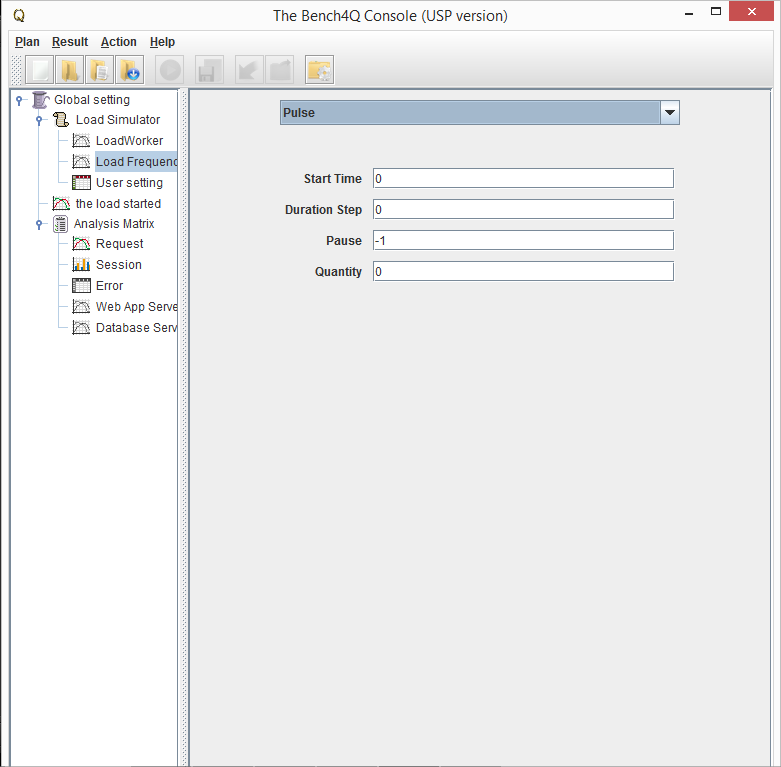
\includegraphics[scale=0.6]{console-bench4Q-usp.png}
	\caption{Console de programação de carga de trabalho.}
	\label{fig:interface-criada-beanch4q}
	\fautor
\end{figure}

A carga de trabalho é imposta ao sistema por meio de requisições HTTP enviadas pelos EBs ao SUT que são executadas nos servidores de aplicação das máquinas virtuais instanciadas no \textit{host}. Essas requisições exigem que as máquinas virtuais se ocupem pelo tempo necessário para processá-las, alterando o desempenho experimentado pelo sistema.
Segundo \citeonline{Nobile2013}, existem dois fatores que envolvem uma requisição e que afetam diretamente o desempenho do sistema:
\begin{citacao}
	o tempo de processamento e a quantidade de carga imposta pelas requisições, são dados pelo tempo de processamento e pela taxa de chegada de novas requisições, respectivamente. Com o tempo, a quantidade e o tamanho das requisições podem se alterar, dependendo do perfil de utilização dos usuários que utilizam o serviço naquele momento. Havendo um aumento em algum desses fatores é possível que o desempenho do sistema sofra degradação, podendo, em casos extremos, entrar em colapso.
\end{citacao}

\begin{figure}[!htb]
	\centering
	\begin{subfigure}{\linewidth}
		\centering
		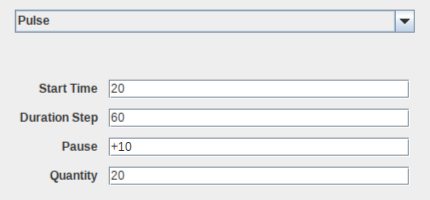
\includegraphics[scale=0.7]{condiguracao-carga-modulada1.png}
		\caption{Teste de configuração da carga a ser modulada}
		\label{fig:configuracao-carga-modulada-teste}
	\end{subfigure}
	
	\begin{subfigure}{\linewidth}
		\centering
		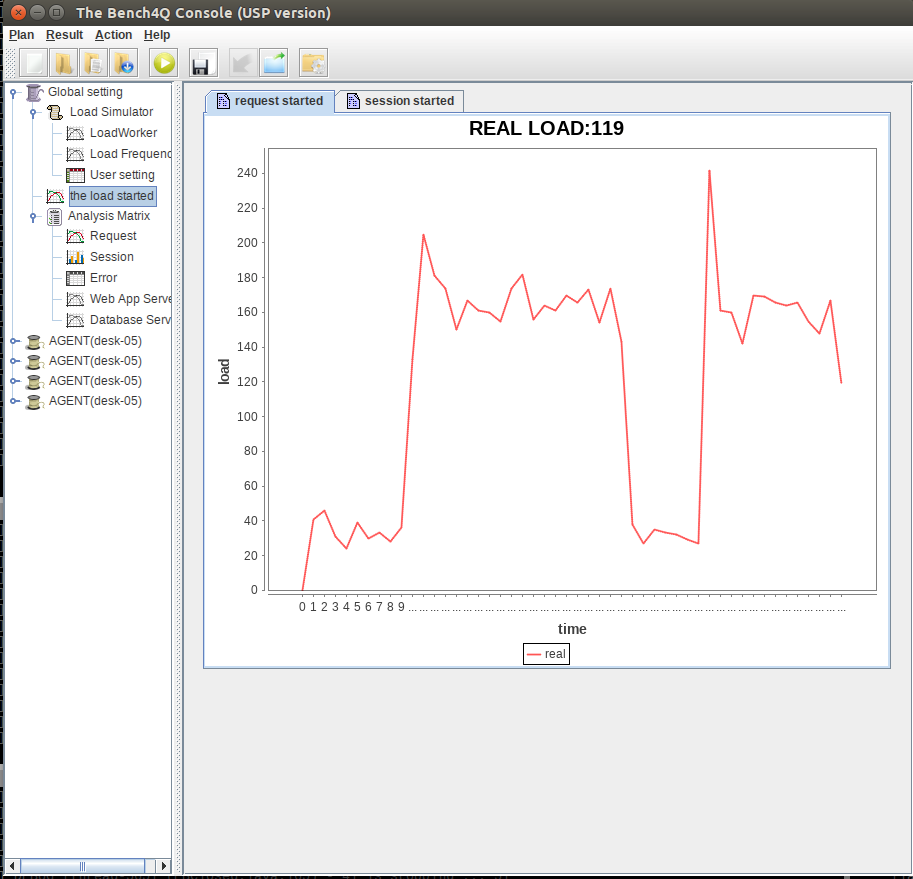
\includegraphics[scale=0.6]{grafico-carga-modulada-teste.png}
		\caption{Carga gerada com base na configuração teste}
		\label{fig:grafico-carga-modulada-teste}
	\end{subfigure}  
	\caption{Teste de modulação da carga}  
	\label{fig:carga-modulada-teste}
	\fautor
\end{figure}  

A Figura \ref{fig:carga-modulada-teste} ilustra uma carga teste modulado já pela extensão, na Figura \ref{fig:configuracao-carga-modulada-teste} apresenta os parâmetros utilizado para fazer o teste, a carga modulada atuará a partir do 10º segundo de experimentação e com uma duração de 20 segundos, com 30 segundos de experimentação ocorrerá uma pausa de 7 segundos e um novo degrau será gerado em seguida, que se manterá até o final do experimento. Para este exemplo foram fixados 40 EBs para modularizar o comportamento da carga. Este comportamento pode ser apreciado no item \ref{fig:grafico-carga-modulada-teste} da mesma figura \ref{fig:carga-modulada-teste}. Vale salientar que o gráfico gerado e apresentado na figura \ref{fig:carga-modulada-teste} de item \ref{fig:grafico-carga-modulada-teste}, é uma característica nativa ao \textit{benchmark}.

O Bench4Q, possui uma documentação sobre a ferramenta. Devido a extensão do \textit{benchmark} foi elaborada uma documentação seguindo os padrões da última versão original e esta pode ser conferida no apêndice A que traz informações do programa e qual seu objetivo, entradas suportadas e saídas esperadas, exemplo de como executar o programa e tabela descrevendo as principais características do mesmo.

\chapter{Resultados}
\label{chapter:resultados}
As análises apresentadas nessa seção resume os resultados dos testes exemplares na extensão feita no Bench4Q, os resultados aqui mostrados são proporcionados como exemplos de aplicação da metodologia, eles não devem ser interpretados como definitivos e avaliações de desempenho. Dessa forma, para uma melhor abordagem dos exemplos apresentados, os exemplo divide-se em 3 partes:
\begin{itemize}
	\item Configuração da carga no Bench4Q
	\item Configuração para modular a carga
	\item Carga gerada
\end{itemize}

\begin{figure}[!htb]
	\begin{subfigure}{\linewidth}
		\centering
		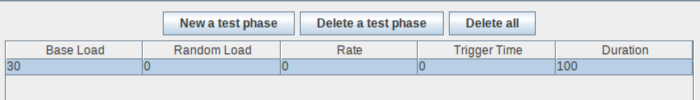
\includegraphics[scale=0.7]{condiguracao-carga-bench4q1.png}
		\caption{Configuração da carga no Bench4Q, para um degrau positivo}
		\label{fig:condiguracao-carga-bench4q1}
	\end{subfigure}\\
	\begin{subfigure}{\linewidth}
		\centering
		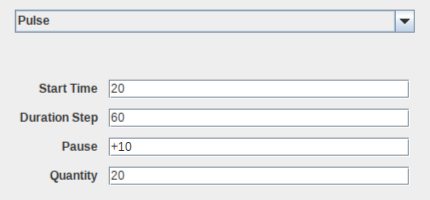
\includegraphics[scale=0.7]{condiguracao-carga-modulada1.png}
		\caption{Configuração para modular a carga como um degrau positivo}
		\label{fig:condiguracao-carga-modulada1}
	\end{subfigure}\\[1ex]
	\begin{subfigure}{\linewidth}
		\centering
		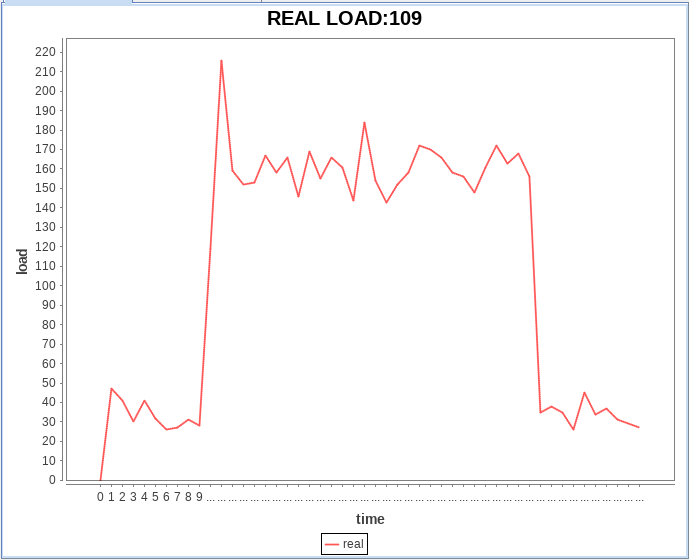
\includegraphics[scale=0.6]{grafico-carga-modulada1.png}
		\caption{Carga gerada com base nas configuração}
		\label{fig:grafico-carga-modulada1}
	\end{subfigure}
	\caption{Carga gerada com base na configuração: Degrau Positivo}
	\label{fig:carga-modulada1}
	\fautor
\end{figure}

A figura \ref{fig:carga-modulada1} apresenta a primeira exemplificação gerada com o Bench4Q já com a extensão desenvolvida neste trabalho, na figura \ref{fig:condiguracao-carga-bench4q1} demonstra os parâmetros de configuração utilizados para gerar a carga, dois são os principiais, \textit{Base Load} e \textit{Duration}, o primeiro define a quantidade e EBs envolvidos nos experimento, neste caso 30 EBs, já o segundo define o tempo de duração do experimento em segundos, neste caso 100 segundos. Na figura \ref{fig:condiguracao-carga-modulada1} são apresentados os parâmetros para modular a carga \textit{Start Time} de valor 20, refere-se ao tempo de esperara para o inicio do restante da carga se mostrar presente e ativa na modulação, assim decorrido 20 segundos os 20, dos 30 EBs, definido pelo \textit{Quantity} iniciam a gerar carga para o sistema, essa carga se manterá ativa durante 60 segundos conforme fixado no parâmetro \textit{Duration Step}, neste exemplo o parâmetro \textit{Pause} não apresentar influencia devido ao seu valor 0.
O resultado pode ser apreciado pela figura \ref{fig:grafico-carga-modulada1}, este gráfico é nativo do próprio Bench4Q, que demonstra o comportamento da carga no decorrer do tempo. Apesar da estocasticidade a carga se modulou conforme programada, essa estocasticidade é característica do Bench4Q, afim de manter um comportamento mais realístico com os de clientes acessando uma estocasticidade \textit{E-commerce}.

\begin{figure}[!htb]
	\begin{subfigure}{\linewidth}
		\centering
		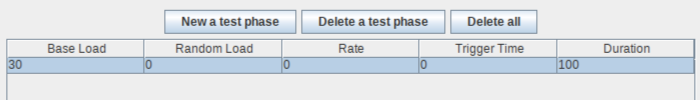
\includegraphics[scale=0.7]{condiguracao-carga-bench4q2.png}
		\caption{Configuração da carga no Bench4Q, para um degrau negativo}
		\label{fig:condiguracao-carga-bench4q2}
	\end{subfigure}\\
	\begin{subfigure}{\linewidth}
		\centering
		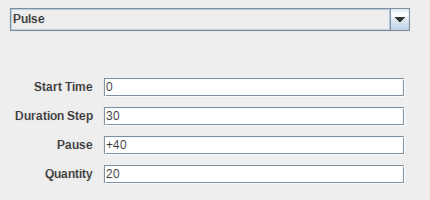
\includegraphics[scale=0.7]{condiguracao-carga-modulada2.png}
		\caption{Configuração para modular a carga como um degrau negativo}
		\label{fig:condiguracao-carga-modulada2}
	\end{subfigure}\\[1ex]
	\begin{subfigure}{\linewidth}
		\centering
		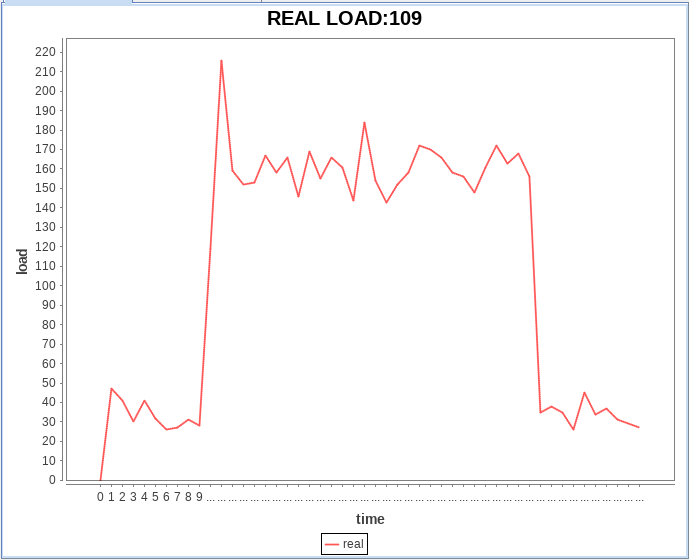
\includegraphics[scale=0.6]{grafico-carga-modulada2.png}
		\caption{Carga gerada com base nas configuração}
		\label{fig:grafico-carga-modulada2}
	\end{subfigure}
	\caption{Carga gerada com base na configuração: Degrau Negativo}
	\label{fig:carga-modulada2}
	\fautor
\end{figure}

A figura \ref{fig:carga-modulada2} apresenta os resultados dos parâmetros para o objetivo do Degrau Negativo. Os parâmetros de \textit{Base Load} e \textit{Duration} são os mesmos do experimento anterior, 30 EBs e 100 segundos de execução, conforme apresentado na figura \ref{fig:condiguracao-carga-bench4q2}. Já na \ref{fig:condiguracao-carga-modulada3} que demonstra os parâmetros utilizados para modular a carga, o \textit{Start Time} recebe o valor 0, assim a carga modulado iniciar com potência máxima utilizando os 30 EBs sendo 20 EBs setado no \textit{Quantity} para reservá-los para a modulação, o tempo de carga máxima é de 30 segundos como é possível ver no parâmetro \textit{Duration Step}, neste caso o \textit{Pause} é setado com 40 segundos, este valor é o que fará a interrupção brusca dos 20 EBs caindo o nível da geração de carga, gerando o degrau negativo. Passado esse período de pausa, a carga retorna ao seu nível máxima e atua por mais 30 segundos, o resultado final pode ser visto na figura \ref{fig:grafico-carga-modulada2}. 
%vale chamar a atenção para a dinâmica apresentada pela geração da carga sempre ao atingir o nivel maximo

\begin{figure}[!htb]
	\begin{subfigure}{\linewidth}
		\centering
		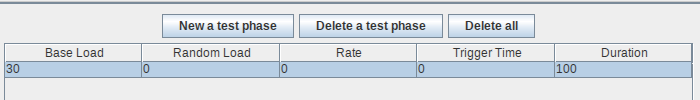
\includegraphics[scale=0.7]{condiguracao-carga-bench4q3.png}
		\caption{Configuração da carga no Bench4Q, para uma onda quadrada}
		\label{fig:condiguracao-carga-bench4q3}
	\end{subfigure}\\
	\begin{subfigure}{\linewidth}
		\centering
		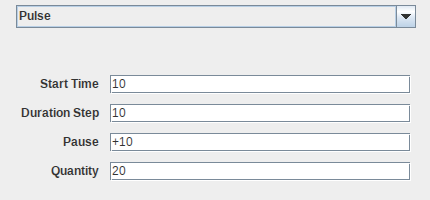
\includegraphics[scale=0.7]{condiguracao-carga-modulada3.png}
		\caption{Configuração para modular a carga como uma onda quadrada}
		\label{fig:condiguracao-carga-modulada3}
	\end{subfigure}\\[1ex]
	\begin{subfigure}{\linewidth}
		\centering
		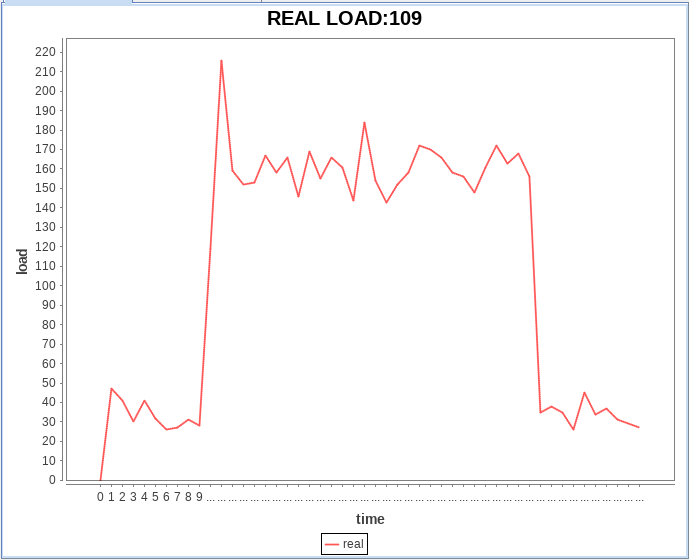
\includegraphics[scale=0.6]{grafico-carga-modulada3.png}
		\caption{Carga gerada com base nas configuração}
		\label{fig:grafico-carga-modulada3}
	\end{subfigure}
	\caption{Carga gerada com base na configuração: Onda Quadrada}
	\label{fig:carga-modulada3}
	\fautor
\end{figure}

Na figura \ref{fig:carga-modulada3} apresenta o resultado a modulação de uma onda quadrada, os parâmetros iniciais do Bench4Q referente a figura \ref{fig:condiguracao-carga-bench4q3} são os mesmos valores dos outros dois exemplos anteriores. Para gerar uma carga modula com comportamento oscilatório como a de uma onda quadrada, os parâmetros \ref{fig:condiguracao-carga-modulada3} são definidos com 10 segundos para \textit{Start Time}, 10 segundo de duração para \textit{Duration Step} e 10 para o \textit{Pause}, também configurado com 20 EBs. Para este exemplo vale salientar que para modular a carga como uma onda quadrada são dois parâmetros são importante e fundamentais \textit{Duration Step} e \textit{Pause}, estes devem ter os mesmos valores, pois eles é o quem manterão durante o período definido a carga em níveis baixo e máximo. 

%3º  - mostrar a analise e o impacto do carga de trabalho no sistema  
%Podemos agora usar os resultados da análise de desempenho para atender as metas estabelecidas no ponto 6.3.1. Por meio do modelo de QPN desenvolvido, que foram capazes de prever o desempenho do sistema em condições de funcionamento normais com 4 e 6 servidores WebLogic. Descobriu-se que usando o balanceador de carga original, seis nós de servidor de aplicação não foram suficientes para garantir tempos médios de resposta de transações de negócios abaixo de meio segundo. Atualizando o balanceador de carga com um CPU ligeiramente mais rápido levou à utilização de CPU do dropping balanceador de carga por um bom 20 por cento.
%Como resultado, os tempos de resposta de transações de concessionários melhorou em 15 a 27 por cento, encontrando o "meio segundo" exigência. No entanto, o aumento da intensidade da carga de trabalho além das condições de pico revelou que o balanceador de carga foi um recurso gargalo, impedindo-nos para escalar o sistema adicionando servidores WebLogic adicionais (veja a Figura 6.14). Assim, à luz do crescimento da carga de trabalho que o esperado, a empresa deve substituir a máquina balanceador de carga com um mais rápido ou considerar o uso de um método de balanceamento de carga mais eficiente. Depois de feito isso, a análise de desempenho deve ser repetida com o novo balanceador de carga para se certificar de que não há nenhum outro gargalos do sistema. Também deve ser assegurado que o balanceador de carga é configurado com threads suficientes para que não há contenção de discussão.
%Neste capítulo, a prática metodologia de modelagem de desempenho para DCS foi apresentada.
%A metodologia aproveita o poder de modelagem e expressividade do formalismo de modelagem QPN para melhorar a representatividade do modelo e permitir a previsão de desempenho precisas. Foi apresentado um estudo de caso detalhado no qual um modelo de um DCS realista foi construído e usado para analisar o seu desempenho e escalabilidade.
%O modelo de representatividade foi validado comparando suas previsões contra medições no sistema real. Foram considerados Um número de diferentes configurações de implantação e cenários de carga de trabalho. Além disso a CPU e I / O de contenção, demonstrou-se como alguns aspectos mais complexas do comportamento do sistema, tais como a contenção de rosca e processamento assíncrono, pode ser modelado. O modelo mostrou para refletir com precisão as características do sistema de desempenho e escalabilidade em estudo. O erro de modelagem para o tempo de resposta da transação não ultrapassou 21,2% e foi muito menor para a transferência de transações e utilização de recursos. A metodologia de modelagem de desempenho proposto fornece uma ferramenta poderosa para a engenharia de DCS desempenho.

%As análises apresentadas nessa Seção consideram a execução de rajadas de requisições dos usuários com e sem a presença de mecanismos de segurança, seguindo o planejamento definido na Seção anterior. Dessa forma, para uma melhor abordagem dos dados analisados, as avaliações foram divididas em duas Seções de acordo com o cenário.

\section{Contribuição}

\chapter{Conclusão}
\label{chapter:conclusao}
A computação em nuvem popularizou um serviço de comercialização se de capacidade computacional na qual a infraestrutura, plataforma ou \textit{software} são ofertados como produto sob demanda e onde os recursos são elásticos, despertando o interesse tanto da comunidade acadêmica quanto da indústria. Atualmente a maioria das grandes soluções de sistemas computacionais são compostas por \textit{mult-tiers}, inclusive quando se refere a aplicações web, devido à flexibilidade de escalabilidade. Para essas aplicações, o planejamento de capacidade é um requisito crítico para determinar a quantidade de recursos exigido para garantia de QoS. No entanto, o planejamento de capacidade é usualmente uma decisão de longo prazo em que, e os recursos são determinados por critérios estáticos. Desta forma, os recursos podem revelar uma sobrecarga em situações de perturbação, mesmo que os níveis de QoS esteja dentro da faixa aceitável para a carga estacionária. %Isso ocorre, devido a utilização da avaliação de desempenho, que é comumente destinada a responder a perguntas estáticas como qual o limite do sistema mediante a uma carga estacionaria imposta. 

Em sistemas que apresentam dinâmica acentuada, a avaliação de desempenho deve considerar que os períodos de regime transiente são importantes. Junto aos mecanismos de elasticidade dos recursos sob demanda, vem a necessidade do autogerenciamento dos recursos. Existem vários trabalhos disponíveis na literatura que lidam e tratam da gestão dos recursos computacionais. Neste trabalho há interesse na modelagem do sistema na forma de uma representação analítica capaz de reproduzir o comportamento dinâmico do sistema, onde o período transiente tem grande colaboração e impacto na política de gerenciamento dos recursos. Um diferencial em relação as abordagens convencionais o objetivo de determinar como a capacidade do sistema em lidar com a variação da carga de trabalho, ao invés de, o desempenho apenas com a carga de trabalho estacionaria.

Mediante a uma arquitetura conceitual proposta por \citeonline{Lourenco2015} e \citeonline{Edwin2015} propõe uma metodologia que descreve e especifica os passos para modelar um sistema computacional por meio de um \textit{benchmark}. No entanto, não foram encontrados \textit{benchmarks} que estimulem a dinâmica do sistema e que permitem uma avaliação em regime transiente, bem como não foram identificados \textit{benchmarks} que sigam a especificação de requisitos proposta por \citeonline{Lourenco2015}.
Este trabalho apresentou uma extensão de um \textit{benchmark}, o Bench4Q, capaz de modelar a sua carga de trabalho de tal maneira a estimular o sistema a apresentar sua dinâmica através da carga. Essa extensão segue um dos requisitos MESC, o modulo \textit{Demand}, proposto por \citeonline{Lourenco2015}, que se restringe a modulação da carga de trabalho, acrescendo-a de provisões para gerar perturbações programadas. Essa extensão, obedece ao padrão de implementação e usabilidade nativas do \textit{benchmark} Bench4Q. A extensão é provida de uma interface gráfica que possibilita a modelagem da carga através da inserção de parâmetros.

Para atingir o objetivo proposto, foi necessária a alteração da carga de trabalho nativa do Bench4Q. Essa modificação resultou na modulação da carga, possibilitando a geração de Degrau Positivo com a carga. Este modelo de carga tem como característica a alteração da sua potência de maneira brusca e repentina. Também é possível gerar um Degrau Negativo que tem efeito oposto ao Degrau Positivo, ou seja, o modelo da carga tem por característica a queda repentina de sua potência. Outra modelagem de carga que a extensão permite é a geração de uma Onda Quadrada, onde existe uma alternância entre os dois modelos descritos anteriormente. 
Por se tratar de um trabalho de extensão de \textit{benchmark} difundido e grande complexidade, as alterações efetuadas trouxeram dificuldades relacionadas a implementação. A falta de uma documentação técnica gerou grande esforço no entendimento e compreensão da implementação original, necessitando muitas vezes a depuração do código para o claro entendimento do seu fluxo de funcionamento tão quando os módulos envolvidos.

O projeto apresentou exemplos práticos das modelagem das cargas propostas (Degrau Positivo, Degrau Negativo e Onda Quadrada) através dos resultados gerados pelo próprio \textit{benchmark}. Os resultados da presente pesquisa foram adequado, na medida em que responderam positivamente ao objetivo do trabalho. O trabalho contemplou uma bateria de experimentos práticos em um ambiente controlado \textit{mult-tier}. Na execução das fases de experimentos, foi elaborado o planejamento do experimento, a coleta de dados e juntamente a análises dos resultados obtidos, resultando em um conjunto de contribuições para a área de pesquisa:
\begin{itemize}
	\item A elaboração de uma documentação padronizada da mesma forma que a original do Bench4Q, contando com versão em inglês que se encontra no apêndice \ref{chapter:documentacao};
	
	\item Impacto da carga modulada: mediante a modulação da carga através da extensão, é possível excitar o sistema a apresentar a sua dinâmica, contribuindo para trabalhos que tem por necessidade a modelagem do sistema e do seu comportamento dinâmico;
	
	\item Dinâmica entre camadas: ao se tratar de um sistema de multicamadas, foi possível perceber, juntamente com a modulação da carga, a dinâmica intrínseca entre as camadas do sistema. Os efeitos combinados de atrasos intrínsecos, ainda que pequenos, e sua propagação por todo as camadas interligados geraram um comportamento dinâmico significante e apreciável;
	
	\item Métrica que mascara: por consequência da dinâmica inerente ao sistema multicamadas, foi possível vislumbrar que nem toda métrica apresenta a realidade quando se lida com um sistema multicamadas. Neste trabalho, foi possível observar esse fato na métrica tempo de resposta.
\end{itemize} 

O presente trabalho foi desenvolvido em consequência aos interesse de estudo da pesquisa de \citeonline{Edwin2015}, e em paralelo a outra iniciativa de \citeonline{Lourenco2015} que especificam a identificação de capacidade dinâmica em sistemas computacionais e como tratá-las com técnicas de modelagem de sistemas. Os resultados do presente trabalho contribuem para ambos os projetos com a disponibilização de um \textit{benchmark} que auxilia na modelagem de sistemas computacionais dinâmicos.

\section{Trabalhos Futuros}
O presente trabalho de mestrado contribuiu para o desenvolvimento de técnicas e estudos interessados na dinâmica do sistema. Todavia, existe uma gama de trilhas a serem exploradas até que a importância da dinâmica de sistemas computacionais tenha maior apreço, como nos casos das ciências e engenharias. Consequentemente este trabalho não finaliza as possibilidades de estudo relacionadas e outros estudos podem ser desenvolvidos a partir dos resultados e constatações identificadas dentre os são:
\begin{itemize}
	\item \textbf{Novas formas de pertubação:} com base nas proposta de \cite{Hellerstein2004} existem outras funções que auxiliam a excitar o sistema a apresentarem a sua dinâmica. 
	
	\item \textbf{Avaliação da dinâmica em sistemas multicamadas:} com o presente trabalho, foi possível observar a dinâmica entre as camadas do sistema, entretanto o presente trabalho não cobre com um planejamento de experimentos utilizando métodos estatísticos por meio de avaliações de desempenho
	
	\item \textbf{Avaliação de métricas de planejamento de recursos em ambiente multicamadas:} este trabalho também revelou que existem métricas que podem mascarar a realidade, neste contexto é importante uma análise das principais métricas de diferentes técnicas para o planejamento de recursos sob um ambiente de multicamadas
\end{itemize} 	


% ---
% Finaliza a parte no bookmark do PDF, para que se inicie o bookmark na raiz
% ---
\bookmarksetup{startatroot}% 
% ---

% ----------------------------------------------------------
% ELEMENTOS PÓS-TEXTUAIS
% ----------------------------------------------------------
\postextual

% ----------------------------------------------------------
% Referências bibliográficas
% ----------------------------------------------------------
\bibliography{../references}

% ---------------------------------------------------------------------
% GLOSSÁRIO
% ---------------------------------------------------------------------

% Arquivo que contém as definições que vão aparecer no glossário
\newword{WYSIWYG}{``What You See Is What You Get''  ou ``O que você vê é o que você obtém''.  Recurso tem por objetivo permitir que um documento, enquanto manipulado na tela, tenha a mesma aparência de sua utilização, usualmente sendo considerada final. Isso facilita para o desenvolvedor que pode trabalhar visualizando a aparência do documento sem precisar salvar em vários momentos e abrir em um \textit{software} separado de visualização}
\newword{Framework}{é uma abstração que une códigos comuns entre vários projetos de \textit{software} provendo uma funcionalidade genérica. \textit{Frameworks} são projetados com a intenção de facilitar o desenvolvimento de \textit{software}, habilitando designers e programadores a gastarem mais tempo determinando as exigências do \textit{software} do que com detalhes de baixo nível do sistema}

\newword{Template}{é um documento sem conteúdo, com apenas a apresentação visual (apenas cabeçalhos por exemplo) e instruções sobre onde e qual tipo de conteúdo deve entrar a cada parcela da apresentação}

\newword{Padrões de projeto}{ou \textit{Design Pattern}, descreve uma solução geral reutilizável para um problema recorrente no desenvolvimento de sistemas de \textit{software} orientados a objetos. Não é um código final, é uma descrição ou modelo de como resolver o problema do qual trata, que pode ser usada em muitas situações diferentes}

\newword{Web}{Sinônimo mais conhecido de \textit{World Wide Web} (WWW). É a interface gráfica da Internet que torna os serviços disponíveis totalmente transparentes para o usuário e ainda possibilita a manipulação multimídia da informação}

% Comando para incluir todas as definições do arquivo glossario.tex
\glsaddall
% Impressão do glossário
\printglossaries

% ----------------------------------------------------------
% Apêndices
% ----------------------------------------------------------

% ---
% Inicia os apêndices
% ---
%\begin{apendicesenv}

%    \chapter{Documento básico usando a classe \textit{icmc}}
%    \label{chapter:documento-basico}
%    
\definecolor{gray}{rgb}{0.4,0.4,0.4}
\definecolor{darkblue}{rgb}{0.0,0.0,0.6}
\definecolor{cyan}{rgb}{0.0,0.6,0.6}
\definecolor{maroon}{rgb}{0.5,0,0}
\definecolor{darkgreen}{rgb}{0,0.5,0}


\lstdefinelanguage{myLatex}
{
    keywords={\titulo},
    alsoletter={-},
    sensitive=false,
    morecomment=[l]{\%},
    morecomment=[s]{/*}{*/},
    morestring=[b]",
    morestring=[b]',
    keywordstyle=\bfseries\color{blue},
    commentstyle=\itshape\color{darkgreen},
    morekeywords={documentclass, titulo, autor, data, orientador, coorientador, curso, textoresumo, incluifichacatalografica, textodedicatoria*, textoagradecimentos*, textoepigrafe*, incluilistadefiguras, incluilistadetabelas, incluilistadequadros, incluilistadealgoritmos, incluilistadecodigos, incluilistadesiglas, incluilistadesimbolos, textual, chapter, postextual, begin, bibliography, end}, 
alsoletter={*, \{, \}, \[, \]},
 morekeywords=[2]{\{, \}, \[, \]},
 keywordstyle=[2]\bfseries\color{blue},
 moredelim=[s][\color{maroon}]{\{}{\}},
    moredelim=[s][\itshape\color{maroon}]{\[}{\]},
}

%\lstdefinelanguage{TeX}
%{
%moredelim=*[s][\color{maroon}]{\{}{\}}
%otherkeywords={\{, \}, \[, \], \\}
%  morestring=[b]",
%  moredelim=[s][\bfseries\color{maroon}]{<}{\ },
%  moredelim=[s][\bfseries\color{maroon}]{</}{>},
%  moredelim=[l][\bfseries\color{maroon}]{/>},
%  moredelim=[l][\bfseries\color{maroon}]{>},
%  commentstyle=\color{darkgreen},
%  stringstyle=\color{blue},
%  identifierstyle=\color{red},
%  keywordstyle=\bfseries\color{maroon}
%moredelim=[l][\bfseries\color{maroon}]{>},
%commentstyle=\color{darkgreen},
%  stringstyle=\color{blue},
%  identifierstyle=\color{red}, moredelim=[l][\bfseries\color{maroon}]{\{},
%  keywordstyle=\bfseries\color{maroon}
%}

%\lstset{language={[LaTeX]TeX},
%texcsstyle=*\bfseries\color{blue},
%keywordstyle=\bfseries\color{blue},
%commentstyle=\color{darkgreen},
%morecomment=[s][\color{red}]{\{}{\}},
%otherkeywords={$, \{, \}, \[, \]}
%}

%\begin{codigo}[caption={Exemplo de um documento básico}, label={codigo:documento-basico}, language={[LaTeX]TeX},  breaklines=true,morekeywords={titulo, autor, data, orientador, coorientador, curso, textoresumo, incluifichacatalografica, textodedicatoria*, textoagradecimentos*, textoepigrafe*, incluilistadefiguras, incluilistadetabelas, incluilistadequadros, incluilistadealgoritmos, incluilistadecodigos, incluilistadesiglas, incluilistadesimbolos, {\backslash}textual, chapter, postextual}, alsoletter={{\backslash},*},morecomment=[s][\color{red}]{\{}{\}}]
\begin{codigo}[caption={Exemplo de um documento básico}, label={codigo:documento-basico}, language={myLatex},  breaklines=true]
% Documento utilizando a classe icmc
% Opções: 
%   Qualificação         = qualificacao 
%   Curso                = doutorado/mestrado
%   Situação do trabalho = pre-defesa/pos-defesa (exceto para qualificação)
% -- opções do pacote babel --
% Idioma padrão = brazil
	%spanish,			% idioma adicional para hifenização
	%english,			% idioma adicional para hifenização
	%brazil				% o último idioma é o principal do documento
\ documentclass[doutorado, spanish, english, brazil]{packages/icmc}

% Título do trabalho
\titulo{Título da Monografia}

% Nome do autor
\autor[Abreviação]{Nome completo do autor}

% Data do depósito
\data{18}{12}{2012}

% Nome do Orientador
\orientador[Orientador]{Titulação do orientador}{Nome completo do Orientador}

% Nome do Coorientador (caso não exista basta remover)
\coorientador[Coorientador]{Titulação do coorientador}{Nome completo do Coorientador}
% Se coorientadora troque Coorientador: por Coorientadora dentro do colchetes

% Sigla do programa de Pós-graduação (CCMC, MAT, PIPGES, PROFMAT, MECAI)
\curso{CCMC}
% O valor entre colchetes é opcional para este programa

% Resumo
\textoresumo[Idioma]{
Texto do resumo do trabalho.
}{Lista de palavras-chave separada por virgulas}

% ----------------------------------------------------------
% ELEMENTOS PRÉ-TEXTUAIS
% ----------------------------------------------------------

% Inserir a ficha catalográfica
\incluifichacatalografica{634} % Código Cutter: número atribuído ao sobrenome do autor (disponível em http://www.davignon.qc.ca/cutter1.html).

% Incluí o texto da Dedicatória
\textodedicatoria*{tex/pre-textual/dedicatoria}

% Incluí o texto dos Agradecimentos
\textoagradecimentos*{tex/pre-textual/agradecimentos}

% Incluí o texto da Epígrafe
\textoepigrafe*{tex/pre-textual/epigrafe}

% Inclui a lista de figuras
\incluilistadefiguras

% Inclui a lista de tabelas
\incluilistadetabelas

% Inclui a lista de quadros
\incluilistadequadros

% Inclui a lista de algoritmos
\incluilistadealgoritmos

% Inclui a lista de códigos
\incluilistadecodigos

% Inclui a lista de siglas e abreviaturas
\incluilistadesiglas

% Inclui a lista de símbolos
\incluilistadesimbolos

% Início do documento
\begin{document}

% ----------------------------------------------------------
% ELEMENTOS TEXTUAIS
% ----------------------------------------------------------
\textual

\chapter{Introdução}

Capítulo de Introdução

\chapter{Desenvolvimento}

Capítulo de Desenvolvimento

\chapter{Conclusão}

Capítulo de conclusão

% ----------------------------------------------------------
% ELEMENTOS PÓS-TEXTUAIS
% ----------------------------------------------------------
\postextual

% Nome do arquivo com as referências bibliográficas
\bibliography{referencias}

\end{document}

\end{codigo}
    
%    \chapter{Configuração do programa JabRef}
%    \label{chapter:configuracao-jabref}
%    \lstdefinelanguage{XML}
{
  morestring=[b]",
  moredelim=[s][\bfseries\color{maroon}]{<}{\ },
  moredelim=[s][\bfseries\color{maroon}]{</}{>},
  moredelim=[l][\bfseries\color{maroon}]{/>},
  moredelim=[l][\bfseries\color{maroon}]{>},
  morecomment=[s]{<?}{?>},
  morecomment=[s]{<!--}{-->},
  commentstyle=\color{darkgreen},
  stringstyle=\color{blue},
  identifierstyle=\color{red}
}


\begin{codigo}[caption={Código de configuração do programa JabRef em XML}, label={codigo:config-jabref}, language=XML, breaklines=true]
<?xml version="1.0" encoding="UTF-8" standalone="no"?>
<!DOCTYPE preferences SYSTEM "http://java.sun.com/dtd/preferences.dtd">
<preferences EXTERNAL_XML_VERSION="1.0">
  <root type="user">
    <map/>
    <node name="net">
      <map/>
      <node name="sf">
        <map/>
        <node name="jabref">
          <map>
            <entry key="KeyPatternRegex" value=""/>
            <entry key="KeyPatternReplacement" value=""/>
            <entry key="abbrAuthorNames" value="true"/>
            <entry key="allowTableEditing" value="false"/>
            <entry key="autoComplete" value="true"/>
            <entry key="autoCompleteFields" value="author;editor;title;journal;publisher;keywords;crossref"/>
            <entry key="autoDoubleBraces" value="true"/>
            <entry key="autoOpenForm" value="true"/>
            <entry key="autoResizeMode" value="4"/>
            <entry key="autoSave" value="true"/>
            <entry key="autoSaveInterval" value="5"/>
            <entry key="autolinkExactKeyOnly" value="true"/>
            <entry key="avoidOverwritingKey" value="false"/>
            <entry key="backup" value="false"/>
            <entry key="caseSensitiveSearch" value="false"/>
            <entry key="citeseerColumn" value="false"/>
            <entry key="confirmDelete" value="true"/>
            <entry key="ctrlClick" value="false"/>
            <entry key="customTypeName_0" value="Article"/>
            <entry key="customTypeName_1" value="Book"/>
            <entry key="customTypeName_10" value="Misc"/>
            <entry key="customTypeName_11" value="Monography"/>
            <entry key="customTypeName_12" value="Patent"/>
            <entry key="customTypeName_13" value="Periodical"/>
            <entry key="customTypeName_14" value="Phdthesis"/>
            <entry key="customTypeName_15" value="Proceedings"/>
            <entry key="customTypeName_16" value="Standard"/>
            <entry key="customTypeName_17" value="Techreport"/>
            <entry key="customTypeName_2" value="Booklet"/>
            <entry key="customTypeName_3" value="Conference"/>
            <entry key="customTypeName_4" value="Electronic"/>
            <entry key="customTypeName_5" value="Inbook"/>
            <entry key="customTypeName_6" value="Incollection"/>
            <entry key="customTypeName_7" value="Inproceedings"/>
            <entry key="customTypeName_8" value="Manual"/>
            <entry key="customTypeName_9" value="Mastersthesis"/>
            <entry key="customTypeOpt_0" value="month;part;section;url;urlaccessdate;note"/>
            <entry key="customTypeOpt_1" value="subtitle;edition;pages;number;series;isbn;volume;org-short;url;urlaccessdate;note"/>
            <entry key="customTypeOpt_10" value="howpublished;month;year;publisher;subtitle;pages;pagename;address;series;number;editortype;url;urlaccessdate;note"/>
            <entry key="customTypeOpt_11" value="pages;pagename;url;urlaccessdate;note"/>
            <entry key="customTypeOpt_12" value="author;title;language;assignee;address;type;number;day;dayfiled;month;monthfiled;url;note"/>
            <entry key="customTypeOpt_13" value="editor;language;series;volume;number;organization;month;url;org-short;note"/>
            <entry key="customTypeOpt_14" value="pages;pagename;url;urlaccessdate;note"/>
            <entry key="customTypeOpt_15" value="editor;volume;number;series;address;publisher;month;organization;org-short;note"/>
            <entry key="customTypeOpt_16" value="author;language;howpublished;type;number;revision;address;month;year;url;org-short;note"/>
            <entry key="customTypeOpt_17" value="pages;pagename;org-short;url;urlaccessdate;number;month;note"/>
            <entry key="customTypeOpt_2" value="subtitle;edition;pages;number;volume;org-short;url;urlaccessdate;note"/>
            <entry key="customTypeOpt_3" value="editor;volume;number;series;pages;address;month;organization;publisher;org-short;note"/>
            <entry key="customTypeOpt_4" value="month;year;org-short;note"/>
            <entry key="customTypeOpt_5" value="booksubtitle;edition;number;series;isbn;volume;org-short;editortype;url;urlaccessdate;note"/>
            <entry key="customTypeOpt_6" value="booksubtitle;edition;number;series;isbn;volume;org-short;editortype;url;urlaccessdate;note"/>
            <entry key="customTypeOpt_7" value="pages;month;publisher;booktitle;conference-location;conference-year;url;urlaccessdate;note"/>
            <entry key="customTypeOpt_8" value="subtitle;author;organization;org-short;address;edition;month;year;pages;series;url;urlaccessdate;note"/>
            <entry key="customTypeOpt_9" value="pages;pagename;url;urlaccessdate;note"/>
            <entry key="customTypeReq_0" value="author;title;journal;year;volume;number;pages"/>
            <entry key="customTypeReq_1" value="title;author/editor/organization;publisher;year;address"/>
            <entry key="customTypeReq_10" value=";author/organization/editor/title"/>
            <entry key="customTypeReq_11" value="author;title;type;school;year;address"/>
            <entry key="customTypeReq_12" value="nationality;number;year;yearfiled"/>
            <entry key="customTypeReq_13" value="title;year"/>
            <entry key="customTypeReq_14" value="author;title;school;year;address"/>
            <entry key="customTypeReq_15" value="title;year"/>
            <entry key="customTypeReq_16" value="title;organization/institution"/>
            <entry key="customTypeReq_17" value="author;title;organization/school;year;address"/>
            <entry key="customTypeReq_2" value="title;author/editor/organization;year"/>
            <entry key="customTypeReq_3" value="author;title;booktitle;year"/>
            <entry key="customTypeReq_4" value="url;urlaccessdate;author/organization/title"/>
            <entry key="customTypeReq_5" value="author;title;editor/organization;booktitle;chapter/pages;publisher;address;year"/>
            <entry key="customTypeReq_6" value="author;title;booktitle;editor/organization;chapter/pages;publisher;address;year"/>
            <entry key="customTypeReq_7" value="author;title;organization;conference-number;year;address"/>
            <entry key="customTypeReq_8" value="title"/>
            <entry key="customTypeReq_9" value="author;title;school;year;address"/>
            <entry key="defaultEncoding" value="ISO8859_15"/>
            <entry key="defaultLabelPattern" value="[auth]:[year]"/>
            <entry key="defaultOwner" value=""/>
            <entry key="defaultShowSource" value="false"/>
            <entry key="dialogWarningForDuplicateKey" value="true"/>
            <entry key="dialogWarningForEmptyKey" value="true"/>
            <entry key="disableOnMultipleSelection" value="false"/>
            <entry key="doNotResolveStringsFor" value="url"/>
            <entry key="enableSourceEditing" value="true"/>
            <entry key="enforceLegalBibtexKey" value="true"/>
            <entry key="exportInOriginalOrder" value="false"/>
            <entry key="exportInStandardOrder" value="true"/>
            <entry key="exportWorkingDirectory" value="/home/marcos/tmp"/>
            <entry key="fileColumn" value="true"/>
            <entry key="fileDirectory" value=""/>
            <entry key="filechooserDisableRename" value="true"/>
            <entry key="floatMarkedEntries" value="true"/>
            <entry key="floatSearch" value="true"/>
            <entry key="fontFamily" value="SansSerif"/>
            <entry key="fontSize" value="12"/>
            <entry key="fontStyle" value="0"/>
            <entry key="generateKeysAfterInspection" value="true"/>
            <entry key="generateKeysBeforeSaving" value="false"/>
            <entry key="gridColor" value="210:210:210"/>
            <entry key="groupAutoHide" value="true"/>
            <entry key="groupAutoShow" value="true"/>
            <entry key="groupExpandTree" value="true"/>
            <entry key="groupKeywordSeparator" value=", "/>
            <entry key="groupShowDynamic" value="true"/>
            <entry key="groupShowIcons" value="true"/>
            <entry key="groupsDefaultField" value="keywords"/>
            <entry key="incompleteEntryBackground" value="250:175:175"/>
            <entry key="incrementS" value="false"/>
            <entry key="lastEdited" value="/home/marcos/Documentos/IFMG/Acadêmico/Aulas/Latex/ifmgbitex/referencias.bib"/>
            <entry key="lastUsedExport" value="html"/>
            <entry key="lookAndFeel" value="com.jgoodies.plaf.plastic.Plastic3DLookAndFeel"/>
            <entry key="markImportedEntries" value="true"/>
            <entry key="markedEntryBackground" value="255:255:180"/>
            <entry key="memoryStickMode" value="false"/>
            <entry key="namesAsIs" value="false"/>
            <entry key="namesFf" value="false"/>
            <entry key="namesLastOnly" value="false"/>
            <entry key="namesNatbib" value="true"/>
            <entry key="openLastEdited" value="true"/>
            <entry key="overrideDefaultFonts" value="false"/>
            <entry key="overwriteOwner" value="false"/>
            <entry key="overwriteTimeStamp" value="false"/>
            <entry key="pdfColumn" value="false"/>
            <entry key="pdfDirectory" value=""/>
            <entry key="posX" value="0"/>
            <entry key="posY" value="0"/>
            <entry key="preview0" value="&lt;font face=&quot;arial&quot;&gt;&lt;b&gt;&lt;i&gt;\bibtextype&lt;/i&gt;&lt;a name=&quot;\bibtexkey&quot;&gt;\begin{bibtexkey} (\bibtexkey)&lt;/a&gt;\end{bibtexkey}&lt;/b&gt;&lt;br&gt;__NEWLINE__\begin{author} \format[HTMLChars,AuthorAbbreviator,AuthorAndsReplacer]{\author}&lt;BR&gt;\end{author}__NEWLINE__\begin{editor} \format[HTMLChars,AuthorAbbreviator,AuthorAndsReplacer]{\editor} &lt;i&gt;(\format[IfPlural(Eds.,Ed.)]{\editor})&lt;/i&gt;&lt;BR&gt;\end{editor}__NEWLINE__\begin{title} \format[HTMLChars]{\title} \end{title}&lt;BR&gt;__NEWLINE__\begin{chapter} \format[HTMLChars]{\chapter}&lt;BR&gt;\end{chapter}__NEWLINE__\begin{journal} &lt;em&gt;\format[HTMLChars]{\journal}, &lt;/em&gt;\end{journal}__NEWLINE__\begin{booktitle} &lt;em&gt;\format[HTMLChars]{\booktitle}, &lt;/em&gt;\end{booktitle}__NEWLINE__\begin{school} &lt;em&gt;\format[HTMLChars]{\school}, &lt;/em&gt;\end{school}__NEWLINE__\begin{institution} &lt;em&gt;\format[HTMLChars]{\institution}, &lt;/em&gt;\end{institution}__NEWLINE__\begin{publisher} &lt;em&gt;\format[HTMLChars]{\publisher}, &lt;/em&gt;\end{publisher}__NEWLINE__\begin{year}&lt;b&gt;\year&lt;/b&gt;\end{year}\begin{volume}&lt;i&gt;, \volume&lt;/i&gt;\end{volume}\begin{pages}, \format[FormatPagesForHTML]{\pages} \end{pages}__NEWLINE__\begin{abstract}&lt;BR&gt;&lt;BR&gt;&lt;b&gt;Abstract: &lt;/b&gt; \format[HTMLChars]{\abstract} \end{abstract}__NEWLINE__\begin{review}&lt;BR&gt;&lt;BR&gt;&lt;b&gt;Review: &lt;/b&gt; \format[HTMLChars]{\review} \end{review}&lt;/dd&gt;__NEWLINE__&lt;p&gt;&lt;/p&gt;&lt;/font&gt;"/>
            <entry key="preview1" value="&lt;font face=&quot;arial&quot;&gt;&lt;b&gt;&lt;i&gt;\bibtextype&lt;/i&gt;&lt;a name=&quot;\bibtexkey&quot;&gt;\begin{bibtexkey} (\bibtexkey)&lt;/a&gt;\end{bibtexkey}&lt;/b&gt;&lt;br&gt;__NEWLINE__\begin{author} \format[HTMLChars,AuthorAbbreviator,AuthorAndsReplacer]{\author}&lt;BR&gt;\end{author}__NEWLINE__\begin{editor} \format[HTMLChars,AuthorAbbreviator,AuthorAndsReplacer]{\editor} &lt;i&gt;(\format[IfPlural(Eds.,Ed.)]{\editor})&lt;/i&gt;&lt;BR&gt;\end{editor}__NEWLINE__\begin{title} \format[HTMLChars]{\title} \end{title}&lt;BR&gt;__NEWLINE__\begin{chapter} \format[HTMLChars]{\chapter}&lt;BR&gt;\end{chapter}__NEWLINE__\begin{journal} &lt;em&gt;\format[HTMLChars]{\journal}, &lt;/em&gt;\end{journal}__NEWLINE__\begin{booktitle} &lt;em&gt;\format[HTMLChars]{\booktitle}, &lt;/em&gt;\end{booktitle}__NEWLINE__\begin{school} &lt;em&gt;\format[HTMLChars]{\school}, &lt;/em&gt;\end{school}__NEWLINE__\begin{institution} &lt;em&gt;\format[HTMLChars]{\institution}, &lt;/em&gt;\end{institution}__NEWLINE__\begin{publisher} &lt;em&gt;\format[HTMLChars]{\publisher}, &lt;/em&gt;\end{publisher}__NEWLINE__\begin{year}&lt;b&gt;\year&lt;/b&gt;\end{year}\begin{volume}&lt;i&gt;, \volume&lt;/i&gt;\end{volume}\begin{pages}, \format[FormatPagesForHTML]{\pages} \end{pages}&lt;/dd&gt;__NEWLINE__&lt;p&gt;&lt;/p&gt;&lt;/font&gt;"/>
            <entry key="priDescending" value="false"/>
            <entry key="priSort" value="entrytype"/>
            <entry key="promptBeforeUsingAutosave" value="true"/>
            <entry key="psDirectory" value=""/>
            <entry key="pushToApplication" value="Insert selected citations into LyX/Kile"/>
            <entry key="recentFiles" value="/home/marcos/Documentos/IFMG/Acadêmico/Aulas/Algoritmos/Algoritmos_exercicios_01/referencias.bib;/home/marcos/Documentos/IFMG/TCC e Projetos/ERP Comparativo/referencias.bib"/>
            <entry key="regExpSearch" value="true"/>
            <entry key="rememberWindowLocation" value="true"/>
            <entry key="resolveStringsAllFields" value="false"/>
            <entry key="runAutomaticFileSearch" value="false"/>
            <entry key="saveInOriginalOrder" value="false"/>
            <entry key="saveInStandardOrder" value="true"/>
            <entry key="searchAll" value="false"/>
            <entry key="searchAllBases" value="false"/>
            <entry key="searchGen" value="true"/>
            <entry key="searchOpt" value="true"/>
            <entry key="searchPanelVisible" value="false"/>
            <entry key="searchReq" value="true"/>
            <entry key="secDescending" value="false"/>
            <entry key="secSort" value=""/>
            <entry key="selectS" value="false"/>
            <entry key="showSearchInDialog" value="false"/>
            <entry key="showSource" value="true"/>
            <entry key="sizeX" value="1280"/>
            <entry key="sizeY" value="800"/>
            <entry key="stringsPosX" value="340"/>
            <entry key="stringsPosY" value="200"/>
            <entry key="stringsSizeX" value="600"/>
            <entry key="stringsSizeY" value="400"/>
            <entry key="tableBackground" value="255:255:255"/>
            <entry key="tableColorCodesOn" value="true"/>
            <entry key="tableOptFieldBackground" value="230:255:230"/>
            <entry key="tableReqFieldBackground" value="230:235:255"/>
            <entry key="tableText" value="0:0:0"/>
            <entry key="terDescending" value="false"/>
            <entry key="terSort" value=""/>
            <entry key="timeStampField" value="timestamp"/>
            <entry key="timeStampFormat" value="dd/MM/yyyy"/>
            <entry key="unmarkAllEntriesBeforeImporting" value="true"/>
            <entry key="urlColumn" value="true"/>
            <entry key="useDefaultLookAndFeel" value="true"/>
            <entry key="useIEEEAbrv" value="true"/>
            <entry key="useImportInspectionDialog" value="true"/>
            <entry key="useImportInspectionDialogForSingle" value="true"/>
            <entry key="useNativeFileDialogOnMac" value="false"/>
            <entry key="useOwner" value="false"/>
            <entry key="useRegExpSearch" value="false"/>
            <entry key="useRemoteServer" value="false"/>
            <entry key="useTimeStamp" value="true"/>
            <entry key="useXmpPrivacyFilter" value="false"/>
            <entry key="warnAboutDuplicatesInInspection" value="true"/>
            <entry key="warnBeforeOverwritingKey" value="true"/>
            <entry key="windowMaximised" value="false"/>
            <entry key="workingDirectory" value="/home/marcos/Documentos/IFMG/Acadêmico/Aulas/Algoritmos/Algoritmos_exercicios_01"/>
          </map>
          <node name="labelPattern">
            <map/>
          </node>
        </node>
      </node>
    </node>
  </root>
</preferences>

\end{codigo}

%\end{apendicesenv}
% ---


% ----------------------------------------------------------
% Anexos
% ----------------------------------------------------------

% ---
% Inicia os anexos
% ---
%\begin{anexosenv}

%    \chapter{Páginas interessantes na Internet} 
%    \label{chapter:paginas-interessantes}
%    \begin{description}
 \item[\url{http://www.tex-br.org}] Página em português com diversos tutoriais e referências interessantes sobre \LaTeX;
 \item[\url{http://en.wikibooks.org/wiki/LaTeX}] Livro em formato \textit{wiki} gratuito sobre \LaTeX;
 \item[\url{http://tobi.oetiker.ch/lshort/lshort.pdf}] Ótimo tutorial sobre \LaTeX (possui versão em português \url{http://alfarrabio.di.uminho.pt/~albie/lshort/ptlshort.pdf}, mas a versão em inglês é a mais atual);
 \item[\url{http://code.google.com/p/abntex2/}] Página do abnTeX2, grupo que desenvolve os pacotes e classes em \LaTeX para as normas da ABNT, nos quais a classe \textit{icmc} foi baseada;
\item[\url{http://www.more.ufsc.br}] Página do Mecanismo On-line para Referências  (MORE) desenvolvido pela UFSC;
\item[\url{http://detexify.kirelabs.org/classify.html}] Página para recuperar o código de símbolos em \LaTeX a partir do desenho fornecido pelo usuário.
 \end{description}

%\end{anexosenv}
% ---

\end{document}